\documentclass[twoside]{book}

% Packages required by doxygen
\usepackage{fixltx2e}
\usepackage{calc}
\usepackage{doxygen}
\usepackage[export]{adjustbox} % also loads graphicx
\usepackage{graphicx}
\usepackage[utf8]{inputenc}
\usepackage{makeidx}
\usepackage{multicol}
\usepackage{multirow}
\PassOptionsToPackage{warn}{textcomp}
\usepackage{textcomp}
\usepackage[nointegrals]{wasysym}
\usepackage[table]{xcolor}

% Font selection
\usepackage[T1]{fontenc}
\usepackage[scaled=.90]{helvet}
\usepackage{courier}
\usepackage{amssymb}
\usepackage{sectsty}
\renewcommand{\familydefault}{\sfdefault}
\allsectionsfont{%
  \fontseries{bc}\selectfont%
  \color{darkgray}%
}
\renewcommand{\DoxyLabelFont}{%
  \fontseries{bc}\selectfont%
  \color{darkgray}%
}
\newcommand{\+}{\discretionary{\mbox{\scriptsize$\hookleftarrow$}}{}{}}

% Page & text layout
\usepackage{geometry}
\geometry{%
  a4paper,%
  top=2.5cm,%
  bottom=2.5cm,%
  left=2.5cm,%
  right=2.5cm%
}
\tolerance=750
\hfuzz=15pt
\hbadness=750
\setlength{\emergencystretch}{15pt}
\setlength{\parindent}{0cm}
\setlength{\parskip}{3ex plus 2ex minus 2ex}
\makeatletter
\renewcommand{\paragraph}{%
  \@startsection{paragraph}{4}{0ex}{-1.0ex}{1.0ex}{%
    \normalfont\normalsize\bfseries\SS@parafont%
  }%
}
\renewcommand{\subparagraph}{%
  \@startsection{subparagraph}{5}{0ex}{-1.0ex}{1.0ex}{%
    \normalfont\normalsize\bfseries\SS@subparafont%
  }%
}
\makeatother

% Headers & footers
\usepackage{fancyhdr}
\pagestyle{fancyplain}
\fancyhead[LE]{\fancyplain{}{\bfseries\thepage}}
\fancyhead[CE]{\fancyplain{}{}}
\fancyhead[RE]{\fancyplain{}{\bfseries\leftmark}}
\fancyhead[LO]{\fancyplain{}{\bfseries\rightmark}}
\fancyhead[CO]{\fancyplain{}{}}
\fancyhead[RO]{\fancyplain{}{\bfseries\thepage}}
\fancyfoot[LE]{\fancyplain{}{}}
\fancyfoot[CE]{\fancyplain{}{}}
\fancyfoot[RE]{\fancyplain{}{\bfseries\scriptsize Generated by Doxygen }}
\fancyfoot[LO]{\fancyplain{}{\bfseries\scriptsize Generated by Doxygen }}
\fancyfoot[CO]{\fancyplain{}{}}
\fancyfoot[RO]{\fancyplain{}{}}
\renewcommand{\footrulewidth}{0.4pt}
\renewcommand{\chaptermark}[1]{%
  \markboth{#1}{}%
}
\renewcommand{\sectionmark}[1]{%
  \markright{\thesection\ #1}%
}

% Indices & bibliography
\usepackage{natbib}
\usepackage[titles]{tocloft}
\setcounter{tocdepth}{3}
\setcounter{secnumdepth}{5}
\makeindex

% Hyperlinks (required, but should be loaded last)
\usepackage{ifpdf}
\ifpdf
  \usepackage[pdftex,pagebackref=true]{hyperref}
\else
  \usepackage[ps2pdf,pagebackref=true]{hyperref}
\fi
\hypersetup{%
  colorlinks=true,%
  linkcolor=blue,%
  citecolor=blue,%
  unicode%
}

% Custom commands
\newcommand{\clearemptydoublepage}{%
  \newpage{\pagestyle{empty}\cleardoublepage}%
}

\usepackage{caption}
\captionsetup{labelsep=space,justification=centering,font={bf},singlelinecheck=off,skip=4pt,position=top}

%===== C O N T E N T S =====

\begin{document}

% Titlepage & ToC
\hypersetup{pageanchor=false,
             bookmarksnumbered=true,
             pdfencoding=unicode
            }
\pagenumbering{alph}
\begin{titlepage}
\vspace*{7cm}
\begin{center}%
{\Large Huffman \\[1ex]\large 1.\+0 }\\
\vspace*{1cm}
{\large Generated by Doxygen 1.8.13}\\
\end{center}
\end{titlepage}
\clearemptydoublepage
\pagenumbering{roman}
\tableofcontents
\clearemptydoublepage
\pagenumbering{arabic}
\hypersetup{pageanchor=true}

%--- Begin generated contents ---
\chapter{H\+U\+F\+F\+M\+AN}
\label{md__r_e_a_d_m_e}
\Hypertarget{md__r_e_a_d_m_e}
\href{https://docs.google.com/document/d/1OUURID_qB3oDBcD7CSMamJLHXSZrWsKi3olc_nWZEvU/edit}{\tt https\+://docs.\+google.\+com/document/d/1\+O\+U\+U\+R\+I\+D\+\_\+q\+B3o\+D\+Bc\+D7\+C\+S\+Mam\+J\+L\+H\+X\+S\+Zr\+Ws\+Ki3olc\+\_\+n\+W\+Z\+Ev\+U/edit} 
\chapter{Data Structure Index}
\section{Data Structures}
Here are the data structures with brief descriptions\+:\begin{DoxyCompactList}
\item\contentsline{section}{\hyperlink{struct_element}{Element} }{\pageref{struct_element}}{}
\item\contentsline{section}{\hyperlink{struct_list___node}{List\+\_\+\+Node} }{\pageref{struct_list___node}}{}
\item\contentsline{section}{\hyperlink{struct_node}{Node} }{\pageref{struct_node}}{}
\end{DoxyCompactList}

\chapter{File Index}
\section{File List}
Here is a list of all files with brief descriptions\+:\begin{DoxyCompactList}
\item\contentsline{section}{\hyperlink{main_8c}{main.\+c} }{\pageref{main_8c}}{}
\item\contentsline{section}{include/\hyperlink{_char_to_binary_8h}{Char\+To\+Binary.\+h} }{\pageref{_char_to_binary_8h}}{}
\item\contentsline{section}{include/\hyperlink{_dictionary_8h}{Dictionary.\+h} }{\pageref{_dictionary_8h}}{}
\item\contentsline{section}{include/\hyperlink{_encoding_8h}{Encoding.\+h} }{\pageref{_encoding_8h}}{}
\item\contentsline{section}{include/\hyperlink{_huffman__tree_8h}{Huffman\+\_\+tree.\+h} }{\pageref{_huffman__tree_8h}}{}
\item\contentsline{section}{include/\hyperlink{_occurrence_8h}{Occurrence.\+h} }{\pageref{_occurrence_8h}}{}
\item\contentsline{section}{src/\hyperlink{_char_to_binary_8c}{Char\+To\+Binary.\+c} }{\pageref{_char_to_binary_8c}}{}
\item\contentsline{section}{src/\hyperlink{_dictionary_8c}{Dictionary.\+c} }{\pageref{_dictionary_8c}}{}
\item\contentsline{section}{src/\hyperlink{_encoding_8c}{Encoding.\+c} }{\pageref{_encoding_8c}}{}
\item\contentsline{section}{src/\hyperlink{_huffman__tree_8c}{Huffman\+\_\+tree.\+c} }{\pageref{_huffman__tree_8c}}{}
\item\contentsline{section}{src/\hyperlink{_occurrence_8c}{Occurrence.\+c} }{\pageref{_occurrence_8c}}{}
\end{DoxyCompactList}

\chapter{Data Structure Documentation}
\hypertarget{struct_element}{}\section{Element Struct Reference}
\label{struct_element}\index{Element@{Element}}


{\ttfamily \#include $<$Occurrence.\+h$>$}



Collaboration diagram for Element\+:\nopagebreak
\begin{figure}[H]
\begin{center}
\leavevmode
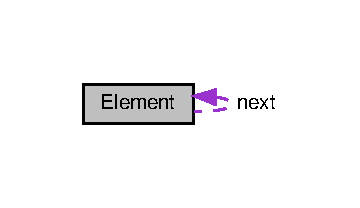
\includegraphics[width=173pt]{struct_element__coll__graph}
\end{center}
\end{figure}
\subsection*{Data Fields}
\begin{DoxyCompactItemize}
\item 
char \hyperlink{struct_element_ac632f0e58c93e01b2bfbb3015c8de34f}{letter}
\item 
int \hyperlink{struct_element_af31c4cdd2ddb799512125a78038c283f}{occ}
\item 
struct \hyperlink{struct_element}{Element} $\ast$ \hyperlink{struct_element_a865f404995b432c38f0626e557399d27}{next}
\end{DoxyCompactItemize}


\subsection{Field Documentation}
\mbox{\Hypertarget{struct_element_ac632f0e58c93e01b2bfbb3015c8de34f}\label{struct_element_ac632f0e58c93e01b2bfbb3015c8de34f}} 
\index{Element@{Element}!letter@{letter}}
\index{letter@{letter}!Element@{Element}}
\subsubsection{\texorpdfstring{letter}{letter}}
{\footnotesize\ttfamily char letter}

the letter contains by the \hyperlink{struct_element}{Element} \mbox{\Hypertarget{struct_element_a865f404995b432c38f0626e557399d27}\label{struct_element_a865f404995b432c38f0626e557399d27}} 
\index{Element@{Element}!next@{next}}
\index{next@{next}!Element@{Element}}
\subsubsection{\texorpdfstring{next}{next}}
{\footnotesize\ttfamily struct \hyperlink{struct_element}{Element}$\ast$ next}

the next \hyperlink{struct_element}{Element} \mbox{\Hypertarget{struct_element_af31c4cdd2ddb799512125a78038c283f}\label{struct_element_af31c4cdd2ddb799512125a78038c283f}} 
\index{Element@{Element}!occ@{occ}}
\index{occ@{occ}!Element@{Element}}
\subsubsection{\texorpdfstring{occ}{occ}}
{\footnotesize\ttfamily int occ}

the occurrence (occ) data 

The documentation for this struct was generated from the following file\+:\begin{DoxyCompactItemize}
\item 
include/\hyperlink{_occurrence_8h}{Occurrence.\+h}\end{DoxyCompactItemize}

\hypertarget{struct_list___node}{}\section{List\+\_\+\+Node Struct Reference}
\label{struct_list___node}\index{List\+\_\+\+Node@{List\+\_\+\+Node}}


{\ttfamily \#include $<$Huffman\+\_\+tree.\+h$>$}



Collaboration diagram for List\+\_\+\+Node\+:\nopagebreak
\begin{figure}[H]
\begin{center}
\leavevmode
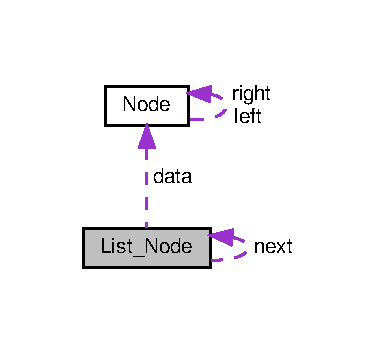
\includegraphics[width=181pt]{struct_list___node__coll__graph}
\end{center}
\end{figure}
\subsection*{Data Fields}
\begin{DoxyCompactItemize}
\item 
struct \hyperlink{struct_list___node}{List\+\_\+\+Node} $\ast$ \hyperlink{struct_list___node_a953735a376f9ca61964264503df3340f}{next}
\item 
\hyperlink{struct_node}{Node} $\ast$ \hyperlink{struct_list___node_a3cf6bebe15c5a482d08f7c9cb9d6fb80}{data}
\end{DoxyCompactItemize}


\subsection{Field Documentation}
\mbox{\Hypertarget{struct_list___node_a3cf6bebe15c5a482d08f7c9cb9d6fb80}\label{struct_list___node_a3cf6bebe15c5a482d08f7c9cb9d6fb80}} 
\index{List\+\_\+\+Node@{List\+\_\+\+Node}!data@{data}}
\index{data@{data}!List\+\_\+\+Node@{List\+\_\+\+Node}}
\subsubsection{\texorpdfstring{data}{data}}
{\footnotesize\ttfamily \hyperlink{struct_node}{Node}$\ast$ data}

the data is a \hyperlink{struct_node}{Node} \mbox{\Hypertarget{struct_list___node_a953735a376f9ca61964264503df3340f}\label{struct_list___node_a953735a376f9ca61964264503df3340f}} 
\index{List\+\_\+\+Node@{List\+\_\+\+Node}!next@{next}}
\index{next@{next}!List\+\_\+\+Node@{List\+\_\+\+Node}}
\subsubsection{\texorpdfstring{next}{next}}
{\footnotesize\ttfamily struct \hyperlink{struct_list___node}{List\+\_\+\+Node}$\ast$ next}

the next \hyperlink{struct_list___node}{List\+\_\+\+Node} 

The documentation for this struct was generated from the following file\+:\begin{DoxyCompactItemize}
\item 
include/\hyperlink{_huffman__tree_8h}{Huffman\+\_\+tree.\+h}\end{DoxyCompactItemize}

\hypertarget{struct_node}{}\section{Node Struct Reference}
\label{struct_node}\index{Node@{Node}}


{\ttfamily \#include $<$Huffman\+\_\+tree.\+h$>$}



Collaboration diagram for Node\+:\nopagebreak
\begin{figure}[H]
\begin{center}
\leavevmode
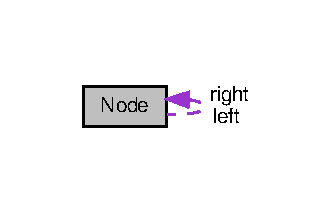
\includegraphics[width=160pt]{struct_node__coll__graph}
\end{center}
\end{figure}
\subsection*{Data Fields}
\begin{DoxyCompactItemize}
\item 
int \hyperlink{struct_node_af31c4cdd2ddb799512125a78038c283f}{occ}
\item 
char \hyperlink{struct_node_ac632f0e58c93e01b2bfbb3015c8de34f}{letter}
\item 
struct \hyperlink{struct_node}{Node} $\ast$ \hyperlink{struct_node_a25eed0b3ce3478a3edb4a00c81dedd5e}{left}
\item 
struct \hyperlink{struct_node}{Node} $\ast$ \hyperlink{struct_node_a760682e46f54442d313a05d18095b52f}{right}
\end{DoxyCompactItemize}


\subsection{Field Documentation}
\mbox{\Hypertarget{struct_node_a25eed0b3ce3478a3edb4a00c81dedd5e}\label{struct_node_a25eed0b3ce3478a3edb4a00c81dedd5e}} 
\index{Node@{Node}!left@{left}}
\index{left@{left}!Node@{Node}}
\subsubsection{\texorpdfstring{left}{left}}
{\footnotesize\ttfamily struct \hyperlink{struct_node}{Node}$\ast$ left}

left child \mbox{\Hypertarget{struct_node_ac632f0e58c93e01b2bfbb3015c8de34f}\label{struct_node_ac632f0e58c93e01b2bfbb3015c8de34f}} 
\index{Node@{Node}!letter@{letter}}
\index{letter@{letter}!Node@{Node}}
\subsubsection{\texorpdfstring{letter}{letter}}
{\footnotesize\ttfamily char letter}

the letter contains by the \hyperlink{struct_element}{Element} \mbox{\Hypertarget{struct_node_af31c4cdd2ddb799512125a78038c283f}\label{struct_node_af31c4cdd2ddb799512125a78038c283f}} 
\index{Node@{Node}!occ@{occ}}
\index{occ@{occ}!Node@{Node}}
\subsubsection{\texorpdfstring{occ}{occ}}
{\footnotesize\ttfamily int occ}

the occurrence (occ) data \mbox{\Hypertarget{struct_node_a760682e46f54442d313a05d18095b52f}\label{struct_node_a760682e46f54442d313a05d18095b52f}} 
\index{Node@{Node}!right@{right}}
\index{right@{right}!Node@{Node}}
\subsubsection{\texorpdfstring{right}{right}}
{\footnotesize\ttfamily struct \hyperlink{struct_node}{Node}$\ast$ right}

right child 

The documentation for this struct was generated from the following file\+:\begin{DoxyCompactItemize}
\item 
include/\hyperlink{_huffman__tree_8h}{Huffman\+\_\+tree.\+h}\end{DoxyCompactItemize}

\chapter{File Documentation}
\hypertarget{_char_to_binary_8h}{}\section{include/\+Char\+To\+Binary.h File Reference}
\label{_char_to_binary_8h}\index{include/\+Char\+To\+Binary.\+h@{include/\+Char\+To\+Binary.\+h}}
This graph shows which files directly or indirectly include this file\+:
\nopagebreak
\begin{figure}[H]
\begin{center}
\leavevmode
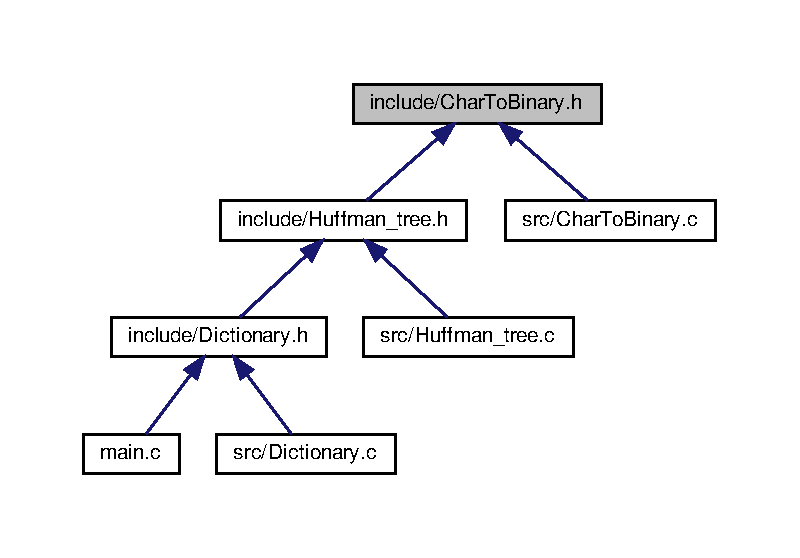
\includegraphics[width=350pt]{_char_to_binary_8h__dep__incl}
\end{center}
\end{figure}
\subsection*{Functions}
\begin{DoxyCompactItemize}
\item 
char $\ast$ \hyperlink{_char_to_binary_8h_ab1ed114c21d39651eb0a80485caba675}{Char\+To\+Binary} (char c)
\begin{DoxyCompactList}\small\item\em convert a char to his binary form. \end{DoxyCompactList}\item 
void \hyperlink{_char_to_binary_8h_a95f18aa97ec5904fef41eb55db53fb5b}{print\+Bin\+Array} (char $\ast$array)
\begin{DoxyCompactList}\small\item\em it print an array only 8 bits array. \end{DoxyCompactList}\item 
void \hyperlink{_char_to_binary_8h_a408cee807a1ce9996877385a21d44aee}{Write\+An\+Array} (F\+I\+LE $\ast$file, char $\ast$array)
\begin{DoxyCompactList}\small\item\em this function write an array in a file.\+txt. \end{DoxyCompactList}\item 
void \hyperlink{_char_to_binary_8h_ad4a8342cc5c08bca70a31d83febbd9ad}{Convert\+Text\+To\+Bin} (char $\ast$texte)
\begin{DoxyCompactList}\small\item\em write the entire text file in binary. \end{DoxyCompactList}\item 
int \hyperlink{_char_to_binary_8h_afaade47ce0269a7de535c4aed8787798}{Char\+Number} (char $\ast$texte)
\begin{DoxyCompactList}\small\item\em Function to count number of character in a file. \end{DoxyCompactList}\end{DoxyCompactItemize}


\subsection{Function Documentation}
\mbox{\Hypertarget{_char_to_binary_8h_afaade47ce0269a7de535c4aed8787798}\label{_char_to_binary_8h_afaade47ce0269a7de535c4aed8787798}} 
\index{Char\+To\+Binary.\+h@{Char\+To\+Binary.\+h}!Char\+Number@{Char\+Number}}
\index{Char\+Number@{Char\+Number}!Char\+To\+Binary.\+h@{Char\+To\+Binary.\+h}}
\subsubsection{\texorpdfstring{Char\+Number()}{CharNumber()}}
{\footnotesize\ttfamily int Char\+Number (\begin{DoxyParamCaption}\item[{char $\ast$}]{texte }\end{DoxyParamCaption})}



Function to count number of character in a file. 


\begin{DoxyParams}{Parameters}
{\em texte.} & \\
\hline
\end{DoxyParams}
\begin{DoxyReturn}{Returns}
int number of character. 
\end{DoxyReturn}
\mbox{\Hypertarget{_char_to_binary_8h_ab1ed114c21d39651eb0a80485caba675}\label{_char_to_binary_8h_ab1ed114c21d39651eb0a80485caba675}} 
\index{Char\+To\+Binary.\+h@{Char\+To\+Binary.\+h}!Char\+To\+Binary@{Char\+To\+Binary}}
\index{Char\+To\+Binary@{Char\+To\+Binary}!Char\+To\+Binary.\+h@{Char\+To\+Binary.\+h}}
\subsubsection{\texorpdfstring{Char\+To\+Binary()}{CharToBinary()}}
{\footnotesize\ttfamily char$\ast$ Char\+To\+Binary (\begin{DoxyParamCaption}\item[{char}]{c }\end{DoxyParamCaption})}



convert a char to his binary form. 


\begin{DoxyParams}{Parameters}
{\em c} & char, one char from the text file. \\
\hline
\end{DoxyParams}
\begin{DoxyReturn}{Returns}
binary array. 
\end{DoxyReturn}
\mbox{\Hypertarget{_char_to_binary_8h_ad4a8342cc5c08bca70a31d83febbd9ad}\label{_char_to_binary_8h_ad4a8342cc5c08bca70a31d83febbd9ad}} 
\index{Char\+To\+Binary.\+h@{Char\+To\+Binary.\+h}!Convert\+Text\+To\+Bin@{Convert\+Text\+To\+Bin}}
\index{Convert\+Text\+To\+Bin@{Convert\+Text\+To\+Bin}!Char\+To\+Binary.\+h@{Char\+To\+Binary.\+h}}
\subsubsection{\texorpdfstring{Convert\+Text\+To\+Bin()}{ConvertTextToBin()}}
{\footnotesize\ttfamily void Convert\+Text\+To\+Bin (\begin{DoxyParamCaption}\item[{char $\ast$}]{texte }\end{DoxyParamCaption})}



write the entire text file in binary. 


\begin{DoxyParams}{Parameters}
{\em texte} & any text file (no N\+U\+LL text). \\
\hline
\end{DoxyParams}
\mbox{\Hypertarget{_char_to_binary_8h_a95f18aa97ec5904fef41eb55db53fb5b}\label{_char_to_binary_8h_a95f18aa97ec5904fef41eb55db53fb5b}} 
\index{Char\+To\+Binary.\+h@{Char\+To\+Binary.\+h}!print\+Bin\+Array@{print\+Bin\+Array}}
\index{print\+Bin\+Array@{print\+Bin\+Array}!Char\+To\+Binary.\+h@{Char\+To\+Binary.\+h}}
\subsubsection{\texorpdfstring{print\+Bin\+Array()}{printBinArray()}}
{\footnotesize\ttfamily void print\+Bin\+Array (\begin{DoxyParamCaption}\item[{char $\ast$}]{array }\end{DoxyParamCaption})}



it print an array only 8 bits array. 


\begin{DoxyParams}{Parameters}
{\em array.} & \\
\hline
\end{DoxyParams}
\mbox{\Hypertarget{_char_to_binary_8h_a408cee807a1ce9996877385a21d44aee}\label{_char_to_binary_8h_a408cee807a1ce9996877385a21d44aee}} 
\index{Char\+To\+Binary.\+h@{Char\+To\+Binary.\+h}!Write\+An\+Array@{Write\+An\+Array}}
\index{Write\+An\+Array@{Write\+An\+Array}!Char\+To\+Binary.\+h@{Char\+To\+Binary.\+h}}
\subsubsection{\texorpdfstring{Write\+An\+Array()}{WriteAnArray()}}
{\footnotesize\ttfamily void Write\+An\+Array (\begin{DoxyParamCaption}\item[{F\+I\+LE $\ast$}]{file,  }\item[{char $\ast$}]{array }\end{DoxyParamCaption})}



this function write an array in a file.\+txt. 

\begin{DoxyNote}{Note}
it only recover array of 8 bits. 
\end{DoxyNote}

\begin{DoxyParams}{Parameters}
{\em file} & file in wich we wanna write. \\
\hline
{\em array} & array of size 7 (0,1,2,3,4,5,6,7). \\
\hline
\end{DoxyParams}

\hypertarget{_dictionary_8h}{}\section{include/\+Dictionary.h File Reference}
\label{_dictionary_8h}\index{include/\+Dictionary.\+h@{include/\+Dictionary.\+h}}
{\ttfamily \#include \char`\"{}Huffman\+\_\+tree.\+h\char`\"{}}\newline
Include dependency graph for Dictionary.\+h\+:
\nopagebreak
\begin{figure}[H]
\begin{center}
\leavevmode
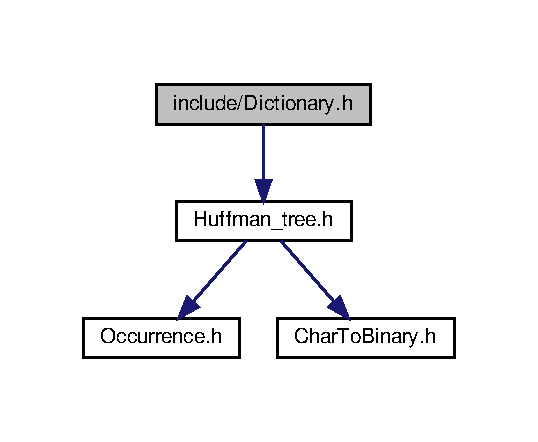
\includegraphics[width=258pt]{_dictionary_8h__incl}
\end{center}
\end{figure}
This graph shows which files directly or indirectly include this file\+:
\nopagebreak
\begin{figure}[H]
\begin{center}
\leavevmode
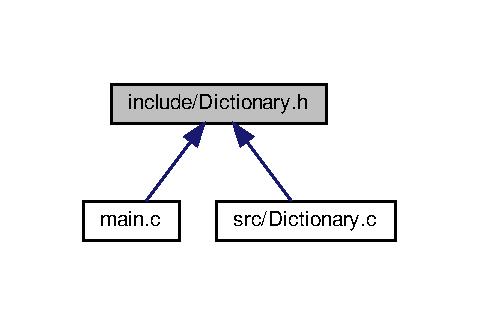
\includegraphics[width=230pt]{_dictionary_8h__dep__incl}
\end{center}
\end{figure}
\subsection*{Functions}
\begin{DoxyCompactItemize}
\item 
void \hyperlink{_dictionary_8h_ae4631a315cca72a95909724d3210a3bf}{Huffman\+Dictionary} (\hyperlink{struct_node}{Node} $\ast$tree, char array\mbox{[}$\,$\mbox{]}, int index)
\begin{DoxyCompactList}\small\item\em create a dictionary from an huffman tree. \end{DoxyCompactList}\item 
void \hyperlink{_dictionary_8h_a092c935ab0fde4b7a4cf4a5b047b9f52}{Write\+Array} (char array\mbox{[}$\,$\mbox{]}, int size, \hyperlink{struct_node}{Node} $\ast$tree)
\begin{DoxyCompactList}\small\item\em Write an array in the dictionary. \end{DoxyCompactList}\item 
unsigned int \hyperlink{_dictionary_8h_a1e4d9bdabe290766cf72727d1de41953}{depth} (\hyperlink{struct_node}{Node} $\ast$tree)
\begin{DoxyCompactList}\small\item\em this function return the depth of any tree. \end{DoxyCompactList}\end{DoxyCompactItemize}


\subsection{Function Documentation}
\mbox{\Hypertarget{_dictionary_8h_a1e4d9bdabe290766cf72727d1de41953}\label{_dictionary_8h_a1e4d9bdabe290766cf72727d1de41953}} 
\index{Dictionary.\+h@{Dictionary.\+h}!depth@{depth}}
\index{depth@{depth}!Dictionary.\+h@{Dictionary.\+h}}
\subsubsection{\texorpdfstring{depth()}{depth()}}
{\footnotesize\ttfamily unsigned int depth (\begin{DoxyParamCaption}\item[{\hyperlink{struct_node}{Node} $\ast$}]{tree }\end{DoxyParamCaption})}



this function return the depth of any tree. 


\begin{DoxyParams}{Parameters}
{\em tree} & a pointer to a tree. \\
\hline
\end{DoxyParams}
\begin{DoxyReturn}{Returns}
depth of the tree. 
\end{DoxyReturn}
\mbox{\Hypertarget{_dictionary_8h_ae4631a315cca72a95909724d3210a3bf}\label{_dictionary_8h_ae4631a315cca72a95909724d3210a3bf}} 
\index{Dictionary.\+h@{Dictionary.\+h}!Huffman\+Dictionary@{Huffman\+Dictionary}}
\index{Huffman\+Dictionary@{Huffman\+Dictionary}!Dictionary.\+h@{Dictionary.\+h}}
\subsubsection{\texorpdfstring{Huffman\+Dictionary()}{HuffmanDictionary()}}
{\footnotesize\ttfamily void Huffman\+Dictionary (\begin{DoxyParamCaption}\item[{\hyperlink{struct_node}{Node} $\ast$}]{tree,  }\item[{char}]{array\mbox{[}$\,$\mbox{]},  }\item[{int}]{index }\end{DoxyParamCaption})}



create a dictionary from an huffman tree. 


\begin{DoxyParams}{Parameters}
{\em tree} & a pointer to an huffman tree. \\
\hline
{\em array} & array that recover the path to a char. \\
\hline
{\em index} & index for the array. \\
\hline
\end{DoxyParams}
\mbox{\Hypertarget{_dictionary_8h_a092c935ab0fde4b7a4cf4a5b047b9f52}\label{_dictionary_8h_a092c935ab0fde4b7a4cf4a5b047b9f52}} 
\index{Dictionary.\+h@{Dictionary.\+h}!Write\+Array@{Write\+Array}}
\index{Write\+Array@{Write\+Array}!Dictionary.\+h@{Dictionary.\+h}}
\subsubsection{\texorpdfstring{Write\+Array()}{WriteArray()}}
{\footnotesize\ttfamily void Write\+Array (\begin{DoxyParamCaption}\item[{char}]{array\mbox{[}$\,$\mbox{]},  }\item[{int}]{size,  }\item[{\hyperlink{struct_node}{Node} $\ast$}]{tree }\end{DoxyParamCaption})}



Write an array in the dictionary. 


\begin{DoxyParams}{Parameters}
{\em array} & array that contain a path to the char. \\
\hline
{\em size} & size of the array. \\
\hline
{\em tree} & a pointer to a tree. \\
\hline
\end{DoxyParams}

\hypertarget{_encoding_8h}{}\section{include/\+Encoding.h File Reference}
\label{_encoding_8h}\index{include/\+Encoding.\+h@{include/\+Encoding.\+h}}
This graph shows which files directly or indirectly include this file\+:
\nopagebreak
\begin{figure}[H]
\begin{center}
\leavevmode
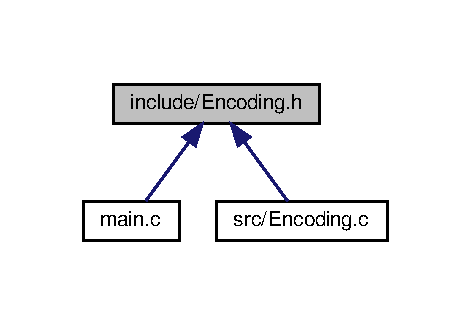
\includegraphics[width=226pt]{_encoding_8h__dep__incl}
\end{center}
\end{figure}
\subsection*{Functions}
\begin{DoxyCompactItemize}
\item 
void \hyperlink{_encoding_8h_a8b56cd79aac05ad82a6e58dab47dcb13}{write\+\_\+huffman\+\_\+text} (F\+I\+LE $\ast$D\+IC, char c)
\begin{DoxyCompactList}\small\item\em Function to write a char into his binary huffman form. \end{DoxyCompactList}\item 
void \hyperlink{_encoding_8h_a68198f3ac4918c84e62d2771b0d8c907}{encoding} ()
\begin{DoxyCompactList}\small\item\em Function to encode a whole text into huffman code. \end{DoxyCompactList}\end{DoxyCompactItemize}


\subsection{Function Documentation}
\mbox{\Hypertarget{_encoding_8h_a68198f3ac4918c84e62d2771b0d8c907}\label{_encoding_8h_a68198f3ac4918c84e62d2771b0d8c907}} 
\index{Encoding.\+h@{Encoding.\+h}!encoding@{encoding}}
\index{encoding@{encoding}!Encoding.\+h@{Encoding.\+h}}
\subsubsection{\texorpdfstring{encoding()}{encoding()}}
{\footnotesize\ttfamily void encoding (\begin{DoxyParamCaption}{ }\end{DoxyParamCaption})}



Function to encode a whole text into huffman code. 

\mbox{\Hypertarget{_encoding_8h_a8b56cd79aac05ad82a6e58dab47dcb13}\label{_encoding_8h_a8b56cd79aac05ad82a6e58dab47dcb13}} 
\index{Encoding.\+h@{Encoding.\+h}!write\+\_\+huffman\+\_\+text@{write\+\_\+huffman\+\_\+text}}
\index{write\+\_\+huffman\+\_\+text@{write\+\_\+huffman\+\_\+text}!Encoding.\+h@{Encoding.\+h}}
\subsubsection{\texorpdfstring{write\+\_\+huffman\+\_\+text()}{write\_huffman\_text()}}
{\footnotesize\ttfamily void write\+\_\+huffman\+\_\+text (\begin{DoxyParamCaption}\item[{F\+I\+LE $\ast$}]{D\+IC,  }\item[{char}]{c }\end{DoxyParamCaption})}



Function to write a char into his binary huffman form. 


\begin{DoxyParams}{Parameters}
{\em D\+IC} & the huffman dictionary. \\
\hline
{\em c} & char want to convert. \\
\hline
\end{DoxyParams}

\hypertarget{_huffman__tree_8h}{}\section{include/\+Huffman\+\_\+tree.h File Reference}
\label{_huffman__tree_8h}\index{include/\+Huffman\+\_\+tree.\+h@{include/\+Huffman\+\_\+tree.\+h}}
{\ttfamily \#include \char`\"{}Occurrence.\+h\char`\"{}}\newline
{\ttfamily \#include \char`\"{}Char\+To\+Binary.\+h\char`\"{}}\newline
Include dependency graph for Huffman\+\_\+tree.\+h\+:
\nopagebreak
\begin{figure}[H]
\begin{center}
\leavevmode
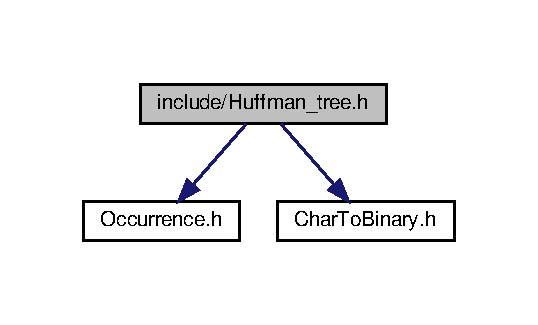
\includegraphics[width=258pt]{_huffman__tree_8h__incl}
\end{center}
\end{figure}
This graph shows which files directly or indirectly include this file\+:
\nopagebreak
\begin{figure}[H]
\begin{center}
\leavevmode
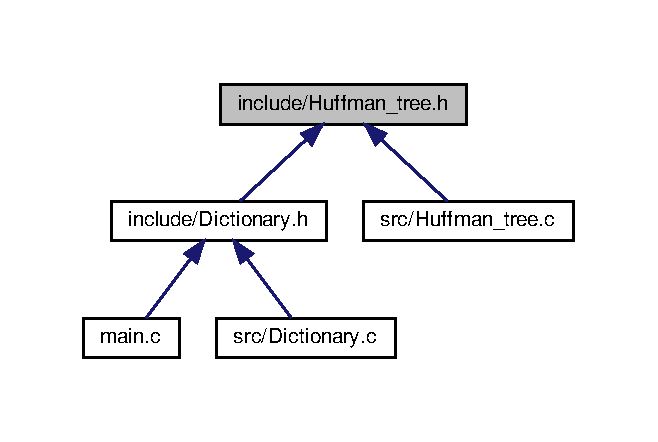
\includegraphics[width=316pt]{_huffman__tree_8h__dep__incl}
\end{center}
\end{figure}
\subsection*{Data Structures}
\begin{DoxyCompactItemize}
\item 
struct \hyperlink{struct_node}{Node}
\item 
struct \hyperlink{struct_list___node}{List\+\_\+\+Node}
\end{DoxyCompactItemize}
\subsection*{Typedefs}
\begin{DoxyCompactItemize}
\item 
typedef struct \hyperlink{struct_node}{Node} \hyperlink{_huffman__tree_8h_a9cf2efdb4ec5c59749c71c81ce1cf726}{Node}
\begin{DoxyCompactList}\small\item\em a \hyperlink{struct_node}{Node} is composed by two pointers \+: left and right. \end{DoxyCompactList}\item 
typedef struct \hyperlink{struct_list___node}{List\+\_\+\+Node} \hyperlink{_huffman__tree_8h_a024953d54075379f88ecaeab243190ba}{List\+\_\+\+Node}
\begin{DoxyCompactList}\small\item\em a \hyperlink{struct_list___node}{List\+\_\+\+Node} is composed by one \hyperlink{struct_node}{Node} and a pointer \+: next. \end{DoxyCompactList}\end{DoxyCompactItemize}
\subsection*{Functions}
\begin{DoxyCompactItemize}
\item 
\hyperlink{struct_list___node}{List\+\_\+\+Node} $\ast$ \hyperlink{_huffman__tree_8h_a0af5331d55b45079167aa5395b32eceb}{min\+\_\+list\+\_\+node} (\hyperlink{struct_list___node}{List\+\_\+\+Node} $\ast$list\+\_\+node)
\begin{DoxyCompactList}\small\item\em Function to find minimum from a \hyperlink{struct_list___node}{List\+\_\+\+Node} List. \end{DoxyCompactList}\item 
void \hyperlink{_huffman__tree_8h_acbf0d3186ab4a1b077a3f0f963bae97f}{list\+\_\+remove\+\_\+node} (\hyperlink{struct_list___node}{List\+\_\+\+Node} $\ast$$\ast$list\+\_\+node, \hyperlink{struct_list___node}{List\+\_\+\+Node} $\ast$min\+\_\+node)
\begin{DoxyCompactList}\small\item\em Function to remove a \hyperlink{struct_list___node}{List\+\_\+\+Node}. \end{DoxyCompactList}\item 
\hyperlink{struct_node}{Node} $\ast$ \hyperlink{_huffman__tree_8h_a9d1186428bbd983ffd985807e40c3a5a}{create\+\_\+\+Node} (\hyperlink{struct_list___node}{List\+\_\+\+Node} $\ast$min1, \hyperlink{struct_list___node}{List\+\_\+\+Node} $\ast$min2)
\begin{DoxyCompactList}\small\item\em Function to create a node with an occurence value equal to sum of two minimum \hyperlink{struct_list___node}{List\+\_\+\+Node} occurrences. \end{DoxyCompactList}\item 
\hyperlink{struct_node}{Node} $\ast$ \hyperlink{_huffman__tree_8h_a97a3db3427a186ef388c738c6b11910f}{create\+\_\+node\+\_\+from\+\_\+element} (\hyperlink{struct_element}{Element} $\ast$element)
\begin{DoxyCompactList}\small\item\em Function to create a node that has been converted from an element. \end{DoxyCompactList}\item 
\hyperlink{struct_list___node}{List\+\_\+\+Node} $\ast$ \hyperlink{_huffman__tree_8h_aaf6def10f6b6a363b0e9b254430312c7}{create\+\_\+list\+\_\+node} (\hyperlink{struct_node}{Node} $\ast$new\+\_\+node)
\begin{DoxyCompactList}\small\item\em Function to create a \hyperlink{struct_list___node}{List\+\_\+\+Node} with a \hyperlink{struct_node}{Node} in parameter. \end{DoxyCompactList}\item 
\hyperlink{struct_list___node}{List\+\_\+\+Node} $\ast$ \hyperlink{_huffman__tree_8h_a99234d1e6e9d21131f06dc7f4ef4919c}{create\+\_\+list\+\_\+node\+\_\+from\+\_\+element} (\hyperlink{struct_element}{Element} $\ast$list)
\begin{DoxyCompactList}\small\item\em Function to create \hyperlink{struct_list___node}{List\+\_\+\+Node} with first element is a \hyperlink{struct_list___node}{List\+\_\+\+Node} element. \end{DoxyCompactList}\item 
\hyperlink{struct_list___node}{List\+\_\+\+Node} $\ast$ \hyperlink{_huffman__tree_8h_a34620fe6b4de52bd588a37a6d9710bb8}{convert\+\_\+elem\+\_\+to\+\_\+\+Node} (\hyperlink{struct_element}{Element} $\ast$list)
\begin{DoxyCompactList}\small\item\em Function to create a List of Liste\+\_\+\+Node from List of \hyperlink{struct_element}{Element}. \end{DoxyCompactList}\item 
void \hyperlink{_huffman__tree_8h_a161297c990d0365c1bdae485b6ee24b9}{Add\+\_\+node\+\_\+beg} (\hyperlink{struct_list___node}{List\+\_\+\+Node} $\ast$$\ast$list\+\_\+node, \hyperlink{struct_node}{Node} $\ast$N\+O\+DE)
\begin{DoxyCompactList}\small\item\em Function to add \hyperlink{struct_list___node}{List\+\_\+\+Node} at the beginning of a \hyperlink{struct_list___node}{List\+\_\+\+Node} List. \end{DoxyCompactList}\item 
void \hyperlink{_huffman__tree_8h_a21fdd931c9da03eef28603b9ff7defd3}{trees\+\_\+log\+\_\+parents\+\_\+before\+\_\+children} (\hyperlink{struct_node}{Node} $\ast$tree)
\begin{DoxyCompactList}\small\item\em Function used to print a tree in prefix order. \end{DoxyCompactList}\item 
\hyperlink{struct_node}{Node} $\ast$ \hyperlink{_huffman__tree_8h_a71663b75a4e86a59c63e43e5eedada53}{huffman\+\_\+tree} (\hyperlink{struct_list___node}{List\+\_\+\+Node} $\ast$list\+\_\+node)
\begin{DoxyCompactList}\small\item\em Function to create an huffman tree. \end{DoxyCompactList}\end{DoxyCompactItemize}


\subsection{Typedef Documentation}
\mbox{\Hypertarget{_huffman__tree_8h_a024953d54075379f88ecaeab243190ba}\label{_huffman__tree_8h_a024953d54075379f88ecaeab243190ba}} 
\index{Huffman\+\_\+tree.\+h@{Huffman\+\_\+tree.\+h}!List\+\_\+\+Node@{List\+\_\+\+Node}}
\index{List\+\_\+\+Node@{List\+\_\+\+Node}!Huffman\+\_\+tree.\+h@{Huffman\+\_\+tree.\+h}}
\subsubsection{\texorpdfstring{List\+\_\+\+Node}{List\_Node}}
{\footnotesize\ttfamily struct \hyperlink{struct_list___node}{List\+\_\+\+Node}}



a \hyperlink{struct_list___node}{List\+\_\+\+Node} is composed by one \hyperlink{struct_node}{Node} and a pointer \+: next. 

\mbox{\Hypertarget{_huffman__tree_8h_a9cf2efdb4ec5c59749c71c81ce1cf726}\label{_huffman__tree_8h_a9cf2efdb4ec5c59749c71c81ce1cf726}} 
\index{Huffman\+\_\+tree.\+h@{Huffman\+\_\+tree.\+h}!Node@{Node}}
\index{Node@{Node}!Huffman\+\_\+tree.\+h@{Huffman\+\_\+tree.\+h}}
\subsubsection{\texorpdfstring{Node}{Node}}
{\footnotesize\ttfamily struct \hyperlink{struct_node}{Node}}



a \hyperlink{struct_node}{Node} is composed by two pointers \+: left and right. 



\subsection{Function Documentation}
\mbox{\Hypertarget{_huffman__tree_8h_a161297c990d0365c1bdae485b6ee24b9}\label{_huffman__tree_8h_a161297c990d0365c1bdae485b6ee24b9}} 
\index{Huffman\+\_\+tree.\+h@{Huffman\+\_\+tree.\+h}!Add\+\_\+node\+\_\+beg@{Add\+\_\+node\+\_\+beg}}
\index{Add\+\_\+node\+\_\+beg@{Add\+\_\+node\+\_\+beg}!Huffman\+\_\+tree.\+h@{Huffman\+\_\+tree.\+h}}
\subsubsection{\texorpdfstring{Add\+\_\+node\+\_\+beg()}{Add\_node\_beg()}}
{\footnotesize\ttfamily void Add\+\_\+node\+\_\+beg (\begin{DoxyParamCaption}\item[{\hyperlink{struct_list___node}{List\+\_\+\+Node} $\ast$$\ast$}]{list\+\_\+node,  }\item[{\hyperlink{struct_node}{Node} $\ast$}]{N\+O\+DE }\end{DoxyParamCaption})}



Function to add \hyperlink{struct_list___node}{List\+\_\+\+Node} at the beginning of a \hyperlink{struct_list___node}{List\+\_\+\+Node} List. 


\begin{DoxyParams}{Parameters}
{\em list\+\_\+node} & a \hyperlink{struct_list___node}{List\+\_\+\+Node} that contain \hyperlink{struct_node}{Node}. \\
\hline
{\em N\+O\+DE} & a \hyperlink{struct_node}{Node} that will become the data of the list\+\_\+node. \\
\hline
\end{DoxyParams}
\mbox{\Hypertarget{_huffman__tree_8h_a34620fe6b4de52bd588a37a6d9710bb8}\label{_huffman__tree_8h_a34620fe6b4de52bd588a37a6d9710bb8}} 
\index{Huffman\+\_\+tree.\+h@{Huffman\+\_\+tree.\+h}!convert\+\_\+elem\+\_\+to\+\_\+\+Node@{convert\+\_\+elem\+\_\+to\+\_\+\+Node}}
\index{convert\+\_\+elem\+\_\+to\+\_\+\+Node@{convert\+\_\+elem\+\_\+to\+\_\+\+Node}!Huffman\+\_\+tree.\+h@{Huffman\+\_\+tree.\+h}}
\subsubsection{\texorpdfstring{convert\+\_\+elem\+\_\+to\+\_\+\+Node()}{convert\_elem\_to\_Node()}}
{\footnotesize\ttfamily \hyperlink{struct_list___node}{List\+\_\+\+Node}$\ast$ convert\+\_\+elem\+\_\+to\+\_\+\+Node (\begin{DoxyParamCaption}\item[{\hyperlink{struct_element}{Element} $\ast$}]{list }\end{DoxyParamCaption})}



Function to create a List of Liste\+\_\+\+Node from List of \hyperlink{struct_element}{Element}. 


\begin{DoxyParams}{Parameters}
{\em list} & a list of element. \\
\hline
\end{DoxyParams}
\begin{DoxyReturn}{Returns}
List\+\_\+\+Node$\ast$ the converted list into \hyperlink{struct_list___node}{List\+\_\+\+Node}. 
\end{DoxyReturn}
\mbox{\Hypertarget{_huffman__tree_8h_aaf6def10f6b6a363b0e9b254430312c7}\label{_huffman__tree_8h_aaf6def10f6b6a363b0e9b254430312c7}} 
\index{Huffman\+\_\+tree.\+h@{Huffman\+\_\+tree.\+h}!create\+\_\+list\+\_\+node@{create\+\_\+list\+\_\+node}}
\index{create\+\_\+list\+\_\+node@{create\+\_\+list\+\_\+node}!Huffman\+\_\+tree.\+h@{Huffman\+\_\+tree.\+h}}
\subsubsection{\texorpdfstring{create\+\_\+list\+\_\+node()}{create\_list\_node()}}
{\footnotesize\ttfamily \hyperlink{struct_list___node}{List\+\_\+\+Node}$\ast$ create\+\_\+list\+\_\+node (\begin{DoxyParamCaption}\item[{\hyperlink{struct_node}{Node} $\ast$}]{new\+\_\+node }\end{DoxyParamCaption})}



Function to create a \hyperlink{struct_list___node}{List\+\_\+\+Node} with a \hyperlink{struct_node}{Node} in parameter. 


\begin{DoxyParams}{Parameters}
{\em new\+\_\+node} & a \hyperlink{struct_node}{Node} pointer. \\
\hline
\end{DoxyParams}
\begin{DoxyReturn}{Returns}
List\+\_\+\+Node$\ast$ a list with a \hyperlink{struct_node}{Node} data. 
\end{DoxyReturn}
\mbox{\Hypertarget{_huffman__tree_8h_a99234d1e6e9d21131f06dc7f4ef4919c}\label{_huffman__tree_8h_a99234d1e6e9d21131f06dc7f4ef4919c}} 
\index{Huffman\+\_\+tree.\+h@{Huffman\+\_\+tree.\+h}!create\+\_\+list\+\_\+node\+\_\+from\+\_\+element@{create\+\_\+list\+\_\+node\+\_\+from\+\_\+element}}
\index{create\+\_\+list\+\_\+node\+\_\+from\+\_\+element@{create\+\_\+list\+\_\+node\+\_\+from\+\_\+element}!Huffman\+\_\+tree.\+h@{Huffman\+\_\+tree.\+h}}
\subsubsection{\texorpdfstring{create\+\_\+list\+\_\+node\+\_\+from\+\_\+element()}{create\_list\_node\_from\_element()}}
{\footnotesize\ttfamily \hyperlink{struct_list___node}{List\+\_\+\+Node}$\ast$ create\+\_\+list\+\_\+node\+\_\+from\+\_\+element (\begin{DoxyParamCaption}\item[{\hyperlink{struct_element}{Element} $\ast$}]{list }\end{DoxyParamCaption})}



Function to create \hyperlink{struct_list___node}{List\+\_\+\+Node} with first element is a \hyperlink{struct_list___node}{List\+\_\+\+Node} element. 


\begin{DoxyParams}{Parameters}
{\em list} & first element of the list. \\
\hline
\end{DoxyParams}
\begin{DoxyReturn}{Returns}
List\+\_\+\+Node$\ast$ the element that has been converted into a \hyperlink{struct_list___node}{List\+\_\+\+Node}. 
\end{DoxyReturn}
\mbox{\Hypertarget{_huffman__tree_8h_a9d1186428bbd983ffd985807e40c3a5a}\label{_huffman__tree_8h_a9d1186428bbd983ffd985807e40c3a5a}} 
\index{Huffman\+\_\+tree.\+h@{Huffman\+\_\+tree.\+h}!create\+\_\+\+Node@{create\+\_\+\+Node}}
\index{create\+\_\+\+Node@{create\+\_\+\+Node}!Huffman\+\_\+tree.\+h@{Huffman\+\_\+tree.\+h}}
\subsubsection{\texorpdfstring{create\+\_\+\+Node()}{create\_Node()}}
{\footnotesize\ttfamily \hyperlink{struct_node}{Node}$\ast$ create\+\_\+\+Node (\begin{DoxyParamCaption}\item[{\hyperlink{struct_list___node}{List\+\_\+\+Node} $\ast$}]{min1,  }\item[{\hyperlink{struct_list___node}{List\+\_\+\+Node} $\ast$}]{min2 }\end{DoxyParamCaption})}



Function to create a node with an occurence value equal to sum of two minimum \hyperlink{struct_list___node}{List\+\_\+\+Node} occurrences. 


\begin{DoxyParams}{Parameters}
{\em min1} & a \hyperlink{struct_list___node}{List\+\_\+\+Node} that contain the first minimum \hyperlink{struct_node}{Node}. \\
\hline
{\em min2} & a \hyperlink{struct_list___node}{List\+\_\+\+Node} that contain the second minimum \hyperlink{struct_node}{Node}. \\
\hline
\end{DoxyParams}
\begin{DoxyReturn}{Returns}
Node$\ast$ the new \hyperlink{struct_node}{Node}. 
\end{DoxyReturn}
\mbox{\Hypertarget{_huffman__tree_8h_a97a3db3427a186ef388c738c6b11910f}\label{_huffman__tree_8h_a97a3db3427a186ef388c738c6b11910f}} 
\index{Huffman\+\_\+tree.\+h@{Huffman\+\_\+tree.\+h}!create\+\_\+node\+\_\+from\+\_\+element@{create\+\_\+node\+\_\+from\+\_\+element}}
\index{create\+\_\+node\+\_\+from\+\_\+element@{create\+\_\+node\+\_\+from\+\_\+element}!Huffman\+\_\+tree.\+h@{Huffman\+\_\+tree.\+h}}
\subsubsection{\texorpdfstring{create\+\_\+node\+\_\+from\+\_\+element()}{create\_node\_from\_element()}}
{\footnotesize\ttfamily \hyperlink{struct_node}{Node}$\ast$ create\+\_\+node\+\_\+from\+\_\+element (\begin{DoxyParamCaption}\item[{\hyperlink{struct_element}{Element} $\ast$}]{element }\end{DoxyParamCaption})}



Function to create a node that has been converted from an element. 


\begin{DoxyParams}{Parameters}
{\em element} & first element to be converted. \\
\hline
\end{DoxyParams}
\begin{DoxyReturn}{Returns}
Node$\ast$ the element that has been converted into a \hyperlink{struct_node}{Node}. 
\end{DoxyReturn}
\mbox{\Hypertarget{_huffman__tree_8h_a71663b75a4e86a59c63e43e5eedada53}\label{_huffman__tree_8h_a71663b75a4e86a59c63e43e5eedada53}} 
\index{Huffman\+\_\+tree.\+h@{Huffman\+\_\+tree.\+h}!huffman\+\_\+tree@{huffman\+\_\+tree}}
\index{huffman\+\_\+tree@{huffman\+\_\+tree}!Huffman\+\_\+tree.\+h@{Huffman\+\_\+tree.\+h}}
\subsubsection{\texorpdfstring{huffman\+\_\+tree()}{huffman\_tree()}}
{\footnotesize\ttfamily \hyperlink{struct_node}{Node}$\ast$ huffman\+\_\+tree (\begin{DoxyParamCaption}\item[{\hyperlink{struct_list___node}{List\+\_\+\+Node} $\ast$}]{list\+\_\+node }\end{DoxyParamCaption})}



Function to create an huffman tree. 


\begin{DoxyParams}{Parameters}
{\em list\+\_\+node} & List that contain all character and their own occurrence. \\
\hline
\end{DoxyParams}
\begin{DoxyReturn}{Returns}
Node$\ast$ the huffman tree. 
\end{DoxyReturn}
\mbox{\Hypertarget{_huffman__tree_8h_acbf0d3186ab4a1b077a3f0f963bae97f}\label{_huffman__tree_8h_acbf0d3186ab4a1b077a3f0f963bae97f}} 
\index{Huffman\+\_\+tree.\+h@{Huffman\+\_\+tree.\+h}!list\+\_\+remove\+\_\+node@{list\+\_\+remove\+\_\+node}}
\index{list\+\_\+remove\+\_\+node@{list\+\_\+remove\+\_\+node}!Huffman\+\_\+tree.\+h@{Huffman\+\_\+tree.\+h}}
\subsubsection{\texorpdfstring{list\+\_\+remove\+\_\+node()}{list\_remove\_node()}}
{\footnotesize\ttfamily void list\+\_\+remove\+\_\+node (\begin{DoxyParamCaption}\item[{\hyperlink{struct_list___node}{List\+\_\+\+Node} $\ast$$\ast$}]{list\+\_\+node,  }\item[{\hyperlink{struct_list___node}{List\+\_\+\+Node} $\ast$}]{min\+\_\+node }\end{DoxyParamCaption})}



Function to remove a \hyperlink{struct_list___node}{List\+\_\+\+Node}. 

\begin{DoxyNote}{Note}
used to remove the minimum. 
\end{DoxyNote}

\begin{DoxyParams}{Parameters}
{\em list\+\_\+node} & a \hyperlink{struct_list___node}{List\+\_\+\+Node} that contain \hyperlink{struct_node}{Node}. \\
\hline
{\em min\+\_\+node} & a \hyperlink{struct_list___node}{List\+\_\+\+Node} that contain the minimum \hyperlink{struct_node}{Node}. \\
\hline
\end{DoxyParams}
\mbox{\Hypertarget{_huffman__tree_8h_a0af5331d55b45079167aa5395b32eceb}\label{_huffman__tree_8h_a0af5331d55b45079167aa5395b32eceb}} 
\index{Huffman\+\_\+tree.\+h@{Huffman\+\_\+tree.\+h}!min\+\_\+list\+\_\+node@{min\+\_\+list\+\_\+node}}
\index{min\+\_\+list\+\_\+node@{min\+\_\+list\+\_\+node}!Huffman\+\_\+tree.\+h@{Huffman\+\_\+tree.\+h}}
\subsubsection{\texorpdfstring{min\+\_\+list\+\_\+node()}{min\_list\_node()}}
{\footnotesize\ttfamily \hyperlink{struct_list___node}{List\+\_\+\+Node}$\ast$ min\+\_\+list\+\_\+node (\begin{DoxyParamCaption}\item[{\hyperlink{struct_list___node}{List\+\_\+\+Node} $\ast$}]{list\+\_\+node }\end{DoxyParamCaption})}



Function to find minimum from a \hyperlink{struct_list___node}{List\+\_\+\+Node} List. 


\begin{DoxyParams}{Parameters}
{\em list\+\_\+node} & a \hyperlink{struct_list___node}{List\+\_\+\+Node} that contain \hyperlink{struct_node}{Node}. \\
\hline
\end{DoxyParams}
\begin{DoxyReturn}{Returns}
List\+\_\+\+Node$\ast$ the minimum occurrence \hyperlink{struct_list___node}{List\+\_\+\+Node}. 
\end{DoxyReturn}
\mbox{\Hypertarget{_huffman__tree_8h_a21fdd931c9da03eef28603b9ff7defd3}\label{_huffman__tree_8h_a21fdd931c9da03eef28603b9ff7defd3}} 
\index{Huffman\+\_\+tree.\+h@{Huffman\+\_\+tree.\+h}!trees\+\_\+log\+\_\+parents\+\_\+before\+\_\+children@{trees\+\_\+log\+\_\+parents\+\_\+before\+\_\+children}}
\index{trees\+\_\+log\+\_\+parents\+\_\+before\+\_\+children@{trees\+\_\+log\+\_\+parents\+\_\+before\+\_\+children}!Huffman\+\_\+tree.\+h@{Huffman\+\_\+tree.\+h}}
\subsubsection{\texorpdfstring{trees\+\_\+log\+\_\+parents\+\_\+before\+\_\+children()}{trees\_log\_parents\_before\_children()}}
{\footnotesize\ttfamily void trees\+\_\+log\+\_\+parents\+\_\+before\+\_\+children (\begin{DoxyParamCaption}\item[{\hyperlink{struct_node}{Node} $\ast$}]{tree }\end{DoxyParamCaption})}



Function used to print a tree in prefix order. 


\begin{DoxyParams}{Parameters}
{\em tree} & a non N\+U\+LL tree. \\
\hline
\end{DoxyParams}

\hypertarget{_occurrence_8h}{}\section{include/\+Occurrence.h File Reference}
\label{_occurrence_8h}\index{include/\+Occurrence.\+h@{include/\+Occurrence.\+h}}
This graph shows which files directly or indirectly include this file\+:
\nopagebreak
\begin{figure}[H]
\begin{center}
\leavevmode
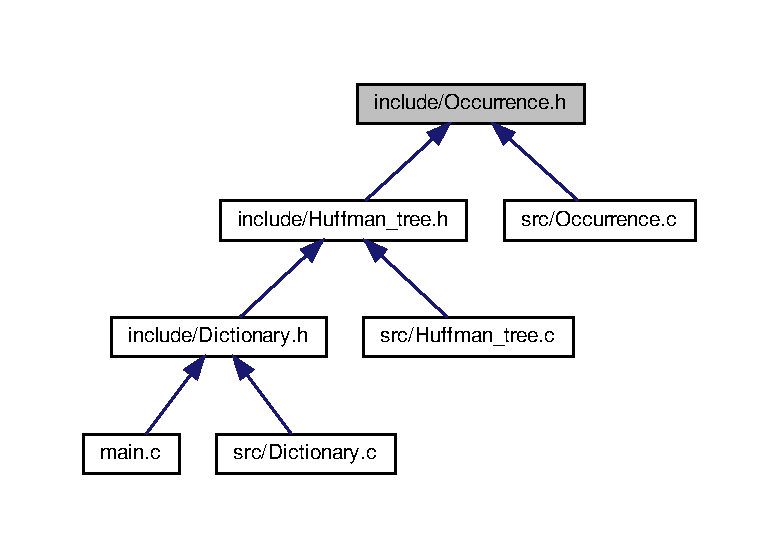
\includegraphics[width=350pt]{_occurrence_8h__dep__incl}
\end{center}
\end{figure}
\subsection*{Data Structures}
\begin{DoxyCompactItemize}
\item 
struct \hyperlink{struct_element}{Element}
\end{DoxyCompactItemize}
\subsection*{Typedefs}
\begin{DoxyCompactItemize}
\item 
typedef struct \hyperlink{struct_element}{Element} \hyperlink{_occurrence_8h_aed98d73ee26a4beb54eaea48f35f8694}{Element}
\begin{DoxyCompactList}\small\item\em \hyperlink{struct_element}{Element} of a list, it owns one pointer \+: next. \end{DoxyCompactList}\end{DoxyCompactItemize}
\subsection*{Functions}
\begin{DoxyCompactItemize}
\item 
\hyperlink{struct_element}{Element} $\ast$ \hyperlink{_occurrence_8h_a7dbd8ad59e7c54573c3cc6554104ec24}{create\+\_\+\+Element} (char letter)
\begin{DoxyCompactList}\small\item\em Create an \hyperlink{struct_element}{Element} object. \end{DoxyCompactList}\item 
void \hyperlink{_occurrence_8h_a7cf8c3bc86fc718bc751012a3ea1bae8}{add\+\_\+occ} (char letter, \hyperlink{struct_element}{Element} $\ast$$\ast$list)
\begin{DoxyCompactList}\small\item\em add one occurrence in the list if the letter exist, else, we create an element at the beginning of the list. \end{DoxyCompactList}\item 
\hyperlink{struct_element}{Element} $\ast$ \hyperlink{_occurrence_8h_a3b8f8fc4b7b66f29fcd36a8e570d65c7}{occurrence} (char $\ast$texte)
\begin{DoxyCompactList}\small\item\em read text file and use add\+\_\+occ to. add letter by letter an occurence to the list of all occurrences. \end{DoxyCompactList}\item 
int \hyperlink{_occurrence_8h_a4a38bc5a9956d58acc78b493668f9e9c}{list\+\_\+size} (\hyperlink{struct_element}{Element} $\ast$l)
\begin{DoxyCompactList}\small\item\em Function who return size of a list. \end{DoxyCompactList}\item 
void \hyperlink{_occurrence_8h_a7bbb9c9a86ff13775d620292f2b29f61}{print\+\_\+list} (\hyperlink{struct_element}{Element} $\ast$list)
\begin{DoxyCompactList}\small\item\em Function to print a list information of a list. \end{DoxyCompactList}\end{DoxyCompactItemize}


\subsection{Typedef Documentation}
\mbox{\Hypertarget{_occurrence_8h_aed98d73ee26a4beb54eaea48f35f8694}\label{_occurrence_8h_aed98d73ee26a4beb54eaea48f35f8694}} 
\index{Occurrence.\+h@{Occurrence.\+h}!Element@{Element}}
\index{Element@{Element}!Occurrence.\+h@{Occurrence.\+h}}
\subsubsection{\texorpdfstring{Element}{Element}}
{\footnotesize\ttfamily struct \hyperlink{struct_element}{Element}}



\hyperlink{struct_element}{Element} of a list, it owns one pointer \+: next. 



\subsection{Function Documentation}
\mbox{\Hypertarget{_occurrence_8h_a7cf8c3bc86fc718bc751012a3ea1bae8}\label{_occurrence_8h_a7cf8c3bc86fc718bc751012a3ea1bae8}} 
\index{Occurrence.\+h@{Occurrence.\+h}!add\+\_\+occ@{add\+\_\+occ}}
\index{add\+\_\+occ@{add\+\_\+occ}!Occurrence.\+h@{Occurrence.\+h}}
\subsubsection{\texorpdfstring{add\+\_\+occ()}{add\_occ()}}
{\footnotesize\ttfamily void add\+\_\+occ (\begin{DoxyParamCaption}\item[{char}]{letter,  }\item[{\hyperlink{struct_element}{Element} $\ast$$\ast$}]{list }\end{DoxyParamCaption})}



add one occurrence in the list if the letter exist, else, we create an element at the beginning of the list. 

\begin{DoxyNote}{Note}
so it modify a list. 
\end{DoxyNote}

\begin{DoxyParams}{Parameters}
{\em letter} & the char to add in the new \hyperlink{struct_element}{Element}. \\
\hline
{\em list} & list we modify,so need double pointer. \\
\hline
\end{DoxyParams}
\mbox{\Hypertarget{_occurrence_8h_a7dbd8ad59e7c54573c3cc6554104ec24}\label{_occurrence_8h_a7dbd8ad59e7c54573c3cc6554104ec24}} 
\index{Occurrence.\+h@{Occurrence.\+h}!create\+\_\+\+Element@{create\+\_\+\+Element}}
\index{create\+\_\+\+Element@{create\+\_\+\+Element}!Occurrence.\+h@{Occurrence.\+h}}
\subsubsection{\texorpdfstring{create\+\_\+\+Element()}{create\_Element()}}
{\footnotesize\ttfamily \hyperlink{struct_element}{Element}$\ast$ create\+\_\+\+Element (\begin{DoxyParamCaption}\item[{char}]{letter }\end{DoxyParamCaption})}



Create an \hyperlink{struct_element}{Element} object. 

\begin{DoxyNote}{Note}
occ initialized at 1. 
\end{DoxyNote}

\begin{DoxyParams}{Parameters}
{\em letter} & the char to add in the new \hyperlink{struct_element}{Element}. \\
\hline
\end{DoxyParams}
\begin{DoxyReturn}{Returns}
Element$\ast$. 
\end{DoxyReturn}
\mbox{\Hypertarget{_occurrence_8h_a4a38bc5a9956d58acc78b493668f9e9c}\label{_occurrence_8h_a4a38bc5a9956d58acc78b493668f9e9c}} 
\index{Occurrence.\+h@{Occurrence.\+h}!list\+\_\+size@{list\+\_\+size}}
\index{list\+\_\+size@{list\+\_\+size}!Occurrence.\+h@{Occurrence.\+h}}
\subsubsection{\texorpdfstring{list\+\_\+size()}{list\_size()}}
{\footnotesize\ttfamily int list\+\_\+size (\begin{DoxyParamCaption}\item[{\hyperlink{struct_element}{Element} $\ast$}]{l }\end{DoxyParamCaption})}



Function who return size of a list. 


\begin{DoxyParams}{Parameters}
{\em l,list} & of \hyperlink{struct_element}{Element}. \\
\hline
\end{DoxyParams}
\begin{DoxyReturn}{Returns}
int, the size of the list. 
\end{DoxyReturn}
\mbox{\Hypertarget{_occurrence_8h_a3b8f8fc4b7b66f29fcd36a8e570d65c7}\label{_occurrence_8h_a3b8f8fc4b7b66f29fcd36a8e570d65c7}} 
\index{Occurrence.\+h@{Occurrence.\+h}!occurrence@{occurrence}}
\index{occurrence@{occurrence}!Occurrence.\+h@{Occurrence.\+h}}
\subsubsection{\texorpdfstring{occurrence()}{occurrence()}}
{\footnotesize\ttfamily \hyperlink{struct_element}{Element}$\ast$ occurrence (\begin{DoxyParamCaption}\item[{char $\ast$}]{texte }\end{DoxyParamCaption})}



read text file and use add\+\_\+occ to. add letter by letter an occurence to the list of all occurrences. 


\begin{DoxyParams}{Parameters}
{\em texte} & file in wich we read char by char. \\
\hline
\end{DoxyParams}
\begin{DoxyReturn}{Returns}
Element$\ast$, the list of all occurrences. 
\end{DoxyReturn}
\mbox{\Hypertarget{_occurrence_8h_a7bbb9c9a86ff13775d620292f2b29f61}\label{_occurrence_8h_a7bbb9c9a86ff13775d620292f2b29f61}} 
\index{Occurrence.\+h@{Occurrence.\+h}!print\+\_\+list@{print\+\_\+list}}
\index{print\+\_\+list@{print\+\_\+list}!Occurrence.\+h@{Occurrence.\+h}}
\subsubsection{\texorpdfstring{print\+\_\+list()}{print\_list()}}
{\footnotesize\ttfamily void print\+\_\+list (\begin{DoxyParamCaption}\item[{\hyperlink{struct_element}{Element} $\ast$}]{list }\end{DoxyParamCaption})}



Function to print a list information of a list. 

\begin{DoxyNote}{Note}
Print letter and number of occurrence. 
\end{DoxyNote}

\begin{DoxyParams}{Parameters}
{\em list,list} & of \hyperlink{struct_element}{Element}. \\
\hline
\end{DoxyParams}

\hypertarget{main_8c}{}\section{main.\+c File Reference}
\label{main_8c}\index{main.\+c@{main.\+c}}
{\ttfamily \#include $<$stdio.\+h$>$}\newline
{\ttfamily \#include $<$stdlib.\+h$>$}\newline
{\ttfamily \#include $<$time.\+h$>$}\newline
{\ttfamily \#include \char`\"{}include/\+Dictionary.\+h\char`\"{}}\newline
{\ttfamily \#include \char`\"{}include/\+Encoding.\+h\char`\"{}}\newline
Include dependency graph for main.\+c\+:
\nopagebreak
\begin{figure}[H]
\begin{center}
\leavevmode
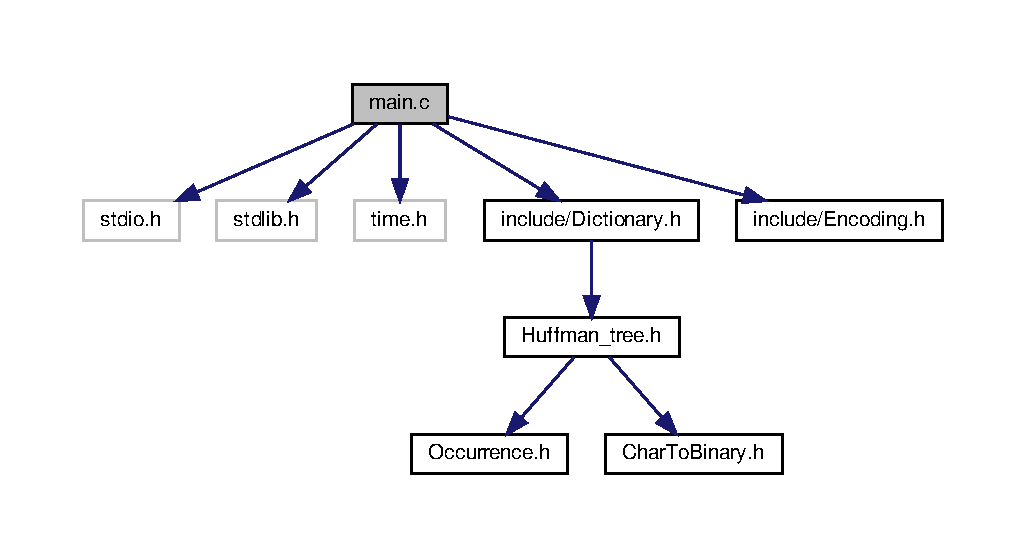
\includegraphics[width=350pt]{main_8c__incl}
\end{center}
\end{figure}
\subsection*{Functions}
\begin{DoxyCompactItemize}
\item 
int \hyperlink{main_8c_ae66f6b31b5ad750f1fe042a706a4e3d4}{main} ()
\end{DoxyCompactItemize}


\subsection{Function Documentation}
\mbox{\Hypertarget{main_8c_ae66f6b31b5ad750f1fe042a706a4e3d4}\label{main_8c_ae66f6b31b5ad750f1fe042a706a4e3d4}} 
\index{main.\+c@{main.\+c}!main@{main}}
\index{main@{main}!main.\+c@{main.\+c}}
\subsubsection{\texorpdfstring{main()}{main()}}
{\footnotesize\ttfamily int main (\begin{DoxyParamCaption}{ }\end{DoxyParamCaption})}


\hypertarget{_r_e_a_d_m_e_8md}{}\section{R\+E\+A\+D\+M\+E.\+md File Reference}
\label{_r_e_a_d_m_e_8md}\index{R\+E\+A\+D\+M\+E.\+md@{R\+E\+A\+D\+M\+E.\+md}}

\hypertarget{_char_to_binary_8c}{}\section{src/\+Char\+To\+Binary.c File Reference}
\label{_char_to_binary_8c}\index{src/\+Char\+To\+Binary.\+c@{src/\+Char\+To\+Binary.\+c}}
{\ttfamily \#include $<$stdio.\+h$>$}\newline
{\ttfamily \#include $<$stdlib.\+h$>$}\newline
{\ttfamily \#include \char`\"{}../include/\+Char\+To\+Binary.\+h\char`\"{}}\newline
Include dependency graph for Char\+To\+Binary.\+c\+:
\nopagebreak
\begin{figure}[H]
\begin{center}
\leavevmode
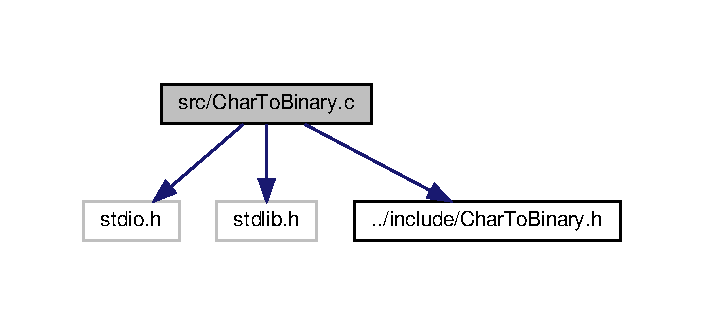
\includegraphics[width=338pt]{_char_to_binary_8c__incl}
\end{center}
\end{figure}
\subsection*{Functions}
\begin{DoxyCompactItemize}
\item 
char $\ast$ \hyperlink{_char_to_binary_8c_ab1ed114c21d39651eb0a80485caba675}{Char\+To\+Binary} (char c)
\begin{DoxyCompactList}\small\item\em convert a char to his binary form. \end{DoxyCompactList}\item 
void \hyperlink{_char_to_binary_8c_a95f18aa97ec5904fef41eb55db53fb5b}{print\+Bin\+Array} (char $\ast$array)
\begin{DoxyCompactList}\small\item\em it print an array only 8 bits array. \end{DoxyCompactList}\item 
void \hyperlink{_char_to_binary_8c_a408cee807a1ce9996877385a21d44aee}{Write\+An\+Array} (F\+I\+LE $\ast$file, char $\ast$array)
\begin{DoxyCompactList}\small\item\em this function write an array in a file.\+txt. \end{DoxyCompactList}\item 
void \hyperlink{_char_to_binary_8c_ad4a8342cc5c08bca70a31d83febbd9ad}{Convert\+Text\+To\+Bin} (char $\ast$texte)
\begin{DoxyCompactList}\small\item\em write the entire text file in binary. \end{DoxyCompactList}\item 
int \hyperlink{_char_to_binary_8c_afaade47ce0269a7de535c4aed8787798}{Char\+Number} (char $\ast$texte)
\begin{DoxyCompactList}\small\item\em Function to count number of character in a file. \end{DoxyCompactList}\end{DoxyCompactItemize}


\subsection{Function Documentation}
\mbox{\Hypertarget{_char_to_binary_8c_afaade47ce0269a7de535c4aed8787798}\label{_char_to_binary_8c_afaade47ce0269a7de535c4aed8787798}} 
\index{Char\+To\+Binary.\+c@{Char\+To\+Binary.\+c}!Char\+Number@{Char\+Number}}
\index{Char\+Number@{Char\+Number}!Char\+To\+Binary.\+c@{Char\+To\+Binary.\+c}}
\subsubsection{\texorpdfstring{Char\+Number()}{CharNumber()}}
{\footnotesize\ttfamily int Char\+Number (\begin{DoxyParamCaption}\item[{char $\ast$}]{texte }\end{DoxyParamCaption})}



Function to count number of character in a file. 


\begin{DoxyParams}{Parameters}
{\em texte.} & \\
\hline
\end{DoxyParams}
\begin{DoxyReturn}{Returns}
int number of character. 
\end{DoxyReturn}
\mbox{\Hypertarget{_char_to_binary_8c_ab1ed114c21d39651eb0a80485caba675}\label{_char_to_binary_8c_ab1ed114c21d39651eb0a80485caba675}} 
\index{Char\+To\+Binary.\+c@{Char\+To\+Binary.\+c}!Char\+To\+Binary@{Char\+To\+Binary}}
\index{Char\+To\+Binary@{Char\+To\+Binary}!Char\+To\+Binary.\+c@{Char\+To\+Binary.\+c}}
\subsubsection{\texorpdfstring{Char\+To\+Binary()}{CharToBinary()}}
{\footnotesize\ttfamily char$\ast$ Char\+To\+Binary (\begin{DoxyParamCaption}\item[{char}]{c }\end{DoxyParamCaption})}



convert a char to his binary form. 


\begin{DoxyParams}{Parameters}
{\em c} & char, one char from the text file. \\
\hline
\end{DoxyParams}
\begin{DoxyReturn}{Returns}
binary array. 
\end{DoxyReturn}
\mbox{\Hypertarget{_char_to_binary_8c_ad4a8342cc5c08bca70a31d83febbd9ad}\label{_char_to_binary_8c_ad4a8342cc5c08bca70a31d83febbd9ad}} 
\index{Char\+To\+Binary.\+c@{Char\+To\+Binary.\+c}!Convert\+Text\+To\+Bin@{Convert\+Text\+To\+Bin}}
\index{Convert\+Text\+To\+Bin@{Convert\+Text\+To\+Bin}!Char\+To\+Binary.\+c@{Char\+To\+Binary.\+c}}
\subsubsection{\texorpdfstring{Convert\+Text\+To\+Bin()}{ConvertTextToBin()}}
{\footnotesize\ttfamily void Convert\+Text\+To\+Bin (\begin{DoxyParamCaption}\item[{char $\ast$}]{texte }\end{DoxyParamCaption})}



write the entire text file in binary. 


\begin{DoxyParams}{Parameters}
{\em texte} & any text file (no N\+U\+LL text). \\
\hline
\end{DoxyParams}
\mbox{\Hypertarget{_char_to_binary_8c_a95f18aa97ec5904fef41eb55db53fb5b}\label{_char_to_binary_8c_a95f18aa97ec5904fef41eb55db53fb5b}} 
\index{Char\+To\+Binary.\+c@{Char\+To\+Binary.\+c}!print\+Bin\+Array@{print\+Bin\+Array}}
\index{print\+Bin\+Array@{print\+Bin\+Array}!Char\+To\+Binary.\+c@{Char\+To\+Binary.\+c}}
\subsubsection{\texorpdfstring{print\+Bin\+Array()}{printBinArray()}}
{\footnotesize\ttfamily void print\+Bin\+Array (\begin{DoxyParamCaption}\item[{char $\ast$}]{array }\end{DoxyParamCaption})}



it print an array only 8 bits array. 


\begin{DoxyParams}{Parameters}
{\em array.} & \\
\hline
\end{DoxyParams}
\mbox{\Hypertarget{_char_to_binary_8c_a408cee807a1ce9996877385a21d44aee}\label{_char_to_binary_8c_a408cee807a1ce9996877385a21d44aee}} 
\index{Char\+To\+Binary.\+c@{Char\+To\+Binary.\+c}!Write\+An\+Array@{Write\+An\+Array}}
\index{Write\+An\+Array@{Write\+An\+Array}!Char\+To\+Binary.\+c@{Char\+To\+Binary.\+c}}
\subsubsection{\texorpdfstring{Write\+An\+Array()}{WriteAnArray()}}
{\footnotesize\ttfamily void Write\+An\+Array (\begin{DoxyParamCaption}\item[{F\+I\+LE $\ast$}]{file,  }\item[{char $\ast$}]{array }\end{DoxyParamCaption})}



this function write an array in a file.\+txt. 

\begin{DoxyNote}{Note}
it only recover array of 8 bits. 
\end{DoxyNote}

\begin{DoxyParams}{Parameters}
{\em file} & file in wich we wanna write. \\
\hline
{\em array} & array of size 7 (0,1,2,3,4,5,6,7). \\
\hline
\end{DoxyParams}

\hypertarget{_dictionary_8c}{}\section{src/\+Dictionary.c File Reference}
\label{_dictionary_8c}\index{src/\+Dictionary.\+c@{src/\+Dictionary.\+c}}
{\ttfamily \#include $<$stdio.\+h$>$}\newline
{\ttfamily \#include $<$stdlib.\+h$>$}\newline
{\ttfamily \#include $<$string.\+h$>$}\newline
{\ttfamily \#include \char`\"{}../include/\+Dictionary.\+h\char`\"{}}\newline
Include dependency graph for Dictionary.\+c\+:
\nopagebreak
\begin{figure}[H]
\begin{center}
\leavevmode
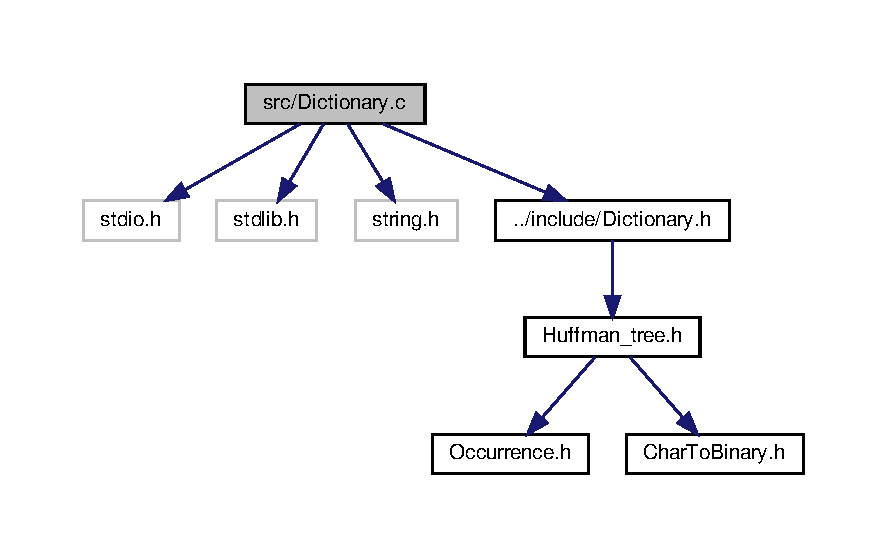
\includegraphics[width=350pt]{_dictionary_8c__incl}
\end{center}
\end{figure}
\subsection*{Functions}
\begin{DoxyCompactItemize}
\item 
void \hyperlink{_dictionary_8c_ae4631a315cca72a95909724d3210a3bf}{Huffman\+Dictionary} (\hyperlink{struct_node}{Node} $\ast$tree, char array\mbox{[}$\,$\mbox{]}, int index)
\begin{DoxyCompactList}\small\item\em create a dictionary from an huffman tree. \end{DoxyCompactList}\item 
void \hyperlink{_dictionary_8c_a092c935ab0fde4b7a4cf4a5b047b9f52}{Write\+Array} (char array\mbox{[}$\,$\mbox{]}, int size, \hyperlink{struct_node}{Node} $\ast$tree)
\begin{DoxyCompactList}\small\item\em Write an array in the dictionary. \end{DoxyCompactList}\item 
unsigned int \hyperlink{_dictionary_8c_a1e4d9bdabe290766cf72727d1de41953}{depth} (\hyperlink{struct_node}{Node} $\ast$tree)
\begin{DoxyCompactList}\small\item\em this function return the depth of any tree. \end{DoxyCompactList}\end{DoxyCompactItemize}


\subsection{Function Documentation}
\mbox{\Hypertarget{_dictionary_8c_a1e4d9bdabe290766cf72727d1de41953}\label{_dictionary_8c_a1e4d9bdabe290766cf72727d1de41953}} 
\index{Dictionary.\+c@{Dictionary.\+c}!depth@{depth}}
\index{depth@{depth}!Dictionary.\+c@{Dictionary.\+c}}
\subsubsection{\texorpdfstring{depth()}{depth()}}
{\footnotesize\ttfamily unsigned int depth (\begin{DoxyParamCaption}\item[{\hyperlink{struct_node}{Node} $\ast$}]{tree }\end{DoxyParamCaption})}



this function return the depth of any tree. 


\begin{DoxyParams}{Parameters}
{\em tree} & a pointer to a tree. \\
\hline
\end{DoxyParams}
\begin{DoxyReturn}{Returns}
depth of the tree. 
\end{DoxyReturn}
\mbox{\Hypertarget{_dictionary_8c_ae4631a315cca72a95909724d3210a3bf}\label{_dictionary_8c_ae4631a315cca72a95909724d3210a3bf}} 
\index{Dictionary.\+c@{Dictionary.\+c}!Huffman\+Dictionary@{Huffman\+Dictionary}}
\index{Huffman\+Dictionary@{Huffman\+Dictionary}!Dictionary.\+c@{Dictionary.\+c}}
\subsubsection{\texorpdfstring{Huffman\+Dictionary()}{HuffmanDictionary()}}
{\footnotesize\ttfamily void Huffman\+Dictionary (\begin{DoxyParamCaption}\item[{\hyperlink{struct_node}{Node} $\ast$}]{tree,  }\item[{char}]{array\mbox{[}$\,$\mbox{]},  }\item[{int}]{index }\end{DoxyParamCaption})}



create a dictionary from an huffman tree. 


\begin{DoxyParams}{Parameters}
{\em tree} & a pointer to an huffman tree. \\
\hline
{\em array} & array that recover the path to a char. \\
\hline
{\em index} & index for the array. \\
\hline
\end{DoxyParams}
\mbox{\Hypertarget{_dictionary_8c_a092c935ab0fde4b7a4cf4a5b047b9f52}\label{_dictionary_8c_a092c935ab0fde4b7a4cf4a5b047b9f52}} 
\index{Dictionary.\+c@{Dictionary.\+c}!Write\+Array@{Write\+Array}}
\index{Write\+Array@{Write\+Array}!Dictionary.\+c@{Dictionary.\+c}}
\subsubsection{\texorpdfstring{Write\+Array()}{WriteArray()}}
{\footnotesize\ttfamily void Write\+Array (\begin{DoxyParamCaption}\item[{char}]{array\mbox{[}$\,$\mbox{]},  }\item[{int}]{size,  }\item[{\hyperlink{struct_node}{Node} $\ast$}]{tree }\end{DoxyParamCaption})}



Write an array in the dictionary. 


\begin{DoxyParams}{Parameters}
{\em array} & array that contain a path to the char. \\
\hline
{\em size} & size of the array. \\
\hline
{\em tree} & a pointer to a tree. \\
\hline
\end{DoxyParams}

\hypertarget{_encoding_8c}{}\section{src/\+Encoding.c File Reference}
\label{_encoding_8c}\index{src/\+Encoding.\+c@{src/\+Encoding.\+c}}
{\ttfamily \#include $<$stdio.\+h$>$}\newline
{\ttfamily \#include $<$stdlib.\+h$>$}\newline
{\ttfamily \#include \char`\"{}../include/\+Encoding.\+h\char`\"{}}\newline
Include dependency graph for Encoding.\+c\+:
\nopagebreak
\begin{figure}[H]
\begin{center}
\leavevmode
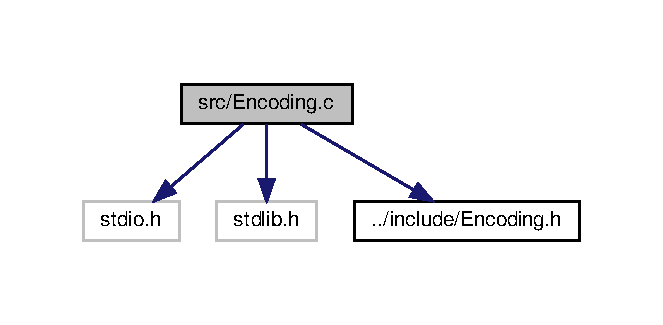
\includegraphics[width=318pt]{_encoding_8c__incl}
\end{center}
\end{figure}
\subsection*{Functions}
\begin{DoxyCompactItemize}
\item 
void \hyperlink{_encoding_8c_a8b56cd79aac05ad82a6e58dab47dcb13}{write\+\_\+huffman\+\_\+text} (F\+I\+LE $\ast$D\+IC, char c)
\begin{DoxyCompactList}\small\item\em Function to write a char into his binary huffman form. \end{DoxyCompactList}\item 
void \hyperlink{_encoding_8c_a68198f3ac4918c84e62d2771b0d8c907}{encoding} ()
\begin{DoxyCompactList}\small\item\em Function to encode a whole text into huffman code. \end{DoxyCompactList}\end{DoxyCompactItemize}


\subsection{Function Documentation}
\mbox{\Hypertarget{_encoding_8c_a68198f3ac4918c84e62d2771b0d8c907}\label{_encoding_8c_a68198f3ac4918c84e62d2771b0d8c907}} 
\index{Encoding.\+c@{Encoding.\+c}!encoding@{encoding}}
\index{encoding@{encoding}!Encoding.\+c@{Encoding.\+c}}
\subsubsection{\texorpdfstring{encoding()}{encoding()}}
{\footnotesize\ttfamily void encoding (\begin{DoxyParamCaption}{ }\end{DoxyParamCaption})}



Function to encode a whole text into huffman code. 

\mbox{\Hypertarget{_encoding_8c_a8b56cd79aac05ad82a6e58dab47dcb13}\label{_encoding_8c_a8b56cd79aac05ad82a6e58dab47dcb13}} 
\index{Encoding.\+c@{Encoding.\+c}!write\+\_\+huffman\+\_\+text@{write\+\_\+huffman\+\_\+text}}
\index{write\+\_\+huffman\+\_\+text@{write\+\_\+huffman\+\_\+text}!Encoding.\+c@{Encoding.\+c}}
\subsubsection{\texorpdfstring{write\+\_\+huffman\+\_\+text()}{write\_huffman\_text()}}
{\footnotesize\ttfamily void write\+\_\+huffman\+\_\+text (\begin{DoxyParamCaption}\item[{F\+I\+LE $\ast$}]{D\+IC,  }\item[{char}]{c }\end{DoxyParamCaption})}



Function to write a char into his binary huffman form. 


\begin{DoxyParams}{Parameters}
{\em D\+IC} & the huffman dictionary. \\
\hline
{\em c} & char want to convert. \\
\hline
\end{DoxyParams}

\hypertarget{_huffman__tree_8c}{}\section{src/\+Huffman\+\_\+tree.c File Reference}
\label{_huffman__tree_8c}\index{src/\+Huffman\+\_\+tree.\+c@{src/\+Huffman\+\_\+tree.\+c}}
{\ttfamily \#include $<$stdio.\+h$>$}\newline
{\ttfamily \#include $<$stdlib.\+h$>$}\newline
{\ttfamily \#include \char`\"{}../include/\+Huffman\+\_\+tree.\+h\char`\"{}}\newline
Include dependency graph for Huffman\+\_\+tree.\+c\+:
\nopagebreak
\begin{figure}[H]
\begin{center}
\leavevmode
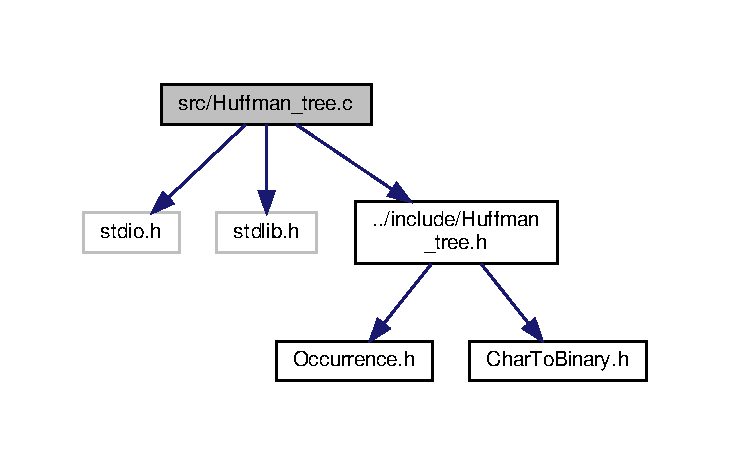
\includegraphics[width=350pt]{_huffman__tree_8c__incl}
\end{center}
\end{figure}
\subsection*{Functions}
\begin{DoxyCompactItemize}
\item 
\hyperlink{struct_list___node}{List\+\_\+\+Node} $\ast$ \hyperlink{_huffman__tree_8c_a0af5331d55b45079167aa5395b32eceb}{min\+\_\+list\+\_\+node} (\hyperlink{struct_list___node}{List\+\_\+\+Node} $\ast$list\+\_\+node)
\begin{DoxyCompactList}\small\item\em Function to find minimum from a \hyperlink{struct_list___node}{List\+\_\+\+Node} List. \end{DoxyCompactList}\item 
void \hyperlink{_huffman__tree_8c_acbf0d3186ab4a1b077a3f0f963bae97f}{list\+\_\+remove\+\_\+node} (\hyperlink{struct_list___node}{List\+\_\+\+Node} $\ast$$\ast$list\+\_\+node, \hyperlink{struct_list___node}{List\+\_\+\+Node} $\ast$min\+\_\+node)
\begin{DoxyCompactList}\small\item\em Function to remove a \hyperlink{struct_list___node}{List\+\_\+\+Node}. \end{DoxyCompactList}\item 
\hyperlink{struct_node}{Node} $\ast$ \hyperlink{_huffman__tree_8c_a9d1186428bbd983ffd985807e40c3a5a}{create\+\_\+\+Node} (\hyperlink{struct_list___node}{List\+\_\+\+Node} $\ast$min1, \hyperlink{struct_list___node}{List\+\_\+\+Node} $\ast$min2)
\begin{DoxyCompactList}\small\item\em Function to create a node with an occurence value equal to sum of two minimum \hyperlink{struct_list___node}{List\+\_\+\+Node} occurrences. \end{DoxyCompactList}\item 
\hyperlink{struct_node}{Node} $\ast$ \hyperlink{_huffman__tree_8c_a97a3db3427a186ef388c738c6b11910f}{create\+\_\+node\+\_\+from\+\_\+element} (\hyperlink{struct_element}{Element} $\ast$element)
\begin{DoxyCompactList}\small\item\em Function to create a node that has been converted from an element. \end{DoxyCompactList}\item 
\hyperlink{struct_list___node}{List\+\_\+\+Node} $\ast$ \hyperlink{_huffman__tree_8c_aaf6def10f6b6a363b0e9b254430312c7}{create\+\_\+list\+\_\+node} (\hyperlink{struct_node}{Node} $\ast$new\+\_\+node)
\begin{DoxyCompactList}\small\item\em Function to create a \hyperlink{struct_list___node}{List\+\_\+\+Node} with a \hyperlink{struct_node}{Node} in parameter. \end{DoxyCompactList}\item 
\hyperlink{struct_list___node}{List\+\_\+\+Node} $\ast$ \hyperlink{_huffman__tree_8c_a99234d1e6e9d21131f06dc7f4ef4919c}{create\+\_\+list\+\_\+node\+\_\+from\+\_\+element} (\hyperlink{struct_element}{Element} $\ast$list)
\begin{DoxyCompactList}\small\item\em Function to create \hyperlink{struct_list___node}{List\+\_\+\+Node} with first element is a \hyperlink{struct_list___node}{List\+\_\+\+Node} element. \end{DoxyCompactList}\item 
\hyperlink{struct_list___node}{List\+\_\+\+Node} $\ast$ \hyperlink{_huffman__tree_8c_a34620fe6b4de52bd588a37a6d9710bb8}{convert\+\_\+elem\+\_\+to\+\_\+\+Node} (\hyperlink{struct_element}{Element} $\ast$list)
\begin{DoxyCompactList}\small\item\em Function to create a List of Liste\+\_\+\+Node from List of \hyperlink{struct_element}{Element}. \end{DoxyCompactList}\item 
void \hyperlink{_huffman__tree_8c_a161297c990d0365c1bdae485b6ee24b9}{Add\+\_\+node\+\_\+beg} (\hyperlink{struct_list___node}{List\+\_\+\+Node} $\ast$$\ast$list\+\_\+node, \hyperlink{struct_node}{Node} $\ast$N\+O\+DE)
\begin{DoxyCompactList}\small\item\em Function to add \hyperlink{struct_list___node}{List\+\_\+\+Node} at the beginning of a \hyperlink{struct_list___node}{List\+\_\+\+Node} List. \end{DoxyCompactList}\item 
void \hyperlink{_huffman__tree_8c_a21fdd931c9da03eef28603b9ff7defd3}{trees\+\_\+log\+\_\+parents\+\_\+before\+\_\+children} (\hyperlink{struct_node}{Node} $\ast$tree)
\begin{DoxyCompactList}\small\item\em Function used to print a tree in prefix order. \end{DoxyCompactList}\item 
\hyperlink{struct_node}{Node} $\ast$ \hyperlink{_huffman__tree_8c_a71663b75a4e86a59c63e43e5eedada53}{huffman\+\_\+tree} (\hyperlink{struct_list___node}{List\+\_\+\+Node} $\ast$list\+\_\+node)
\begin{DoxyCompactList}\small\item\em Function to create an huffman tree. \end{DoxyCompactList}\end{DoxyCompactItemize}


\subsection{Function Documentation}
\mbox{\Hypertarget{_huffman__tree_8c_a161297c990d0365c1bdae485b6ee24b9}\label{_huffman__tree_8c_a161297c990d0365c1bdae485b6ee24b9}} 
\index{Huffman\+\_\+tree.\+c@{Huffman\+\_\+tree.\+c}!Add\+\_\+node\+\_\+beg@{Add\+\_\+node\+\_\+beg}}
\index{Add\+\_\+node\+\_\+beg@{Add\+\_\+node\+\_\+beg}!Huffman\+\_\+tree.\+c@{Huffman\+\_\+tree.\+c}}
\subsubsection{\texorpdfstring{Add\+\_\+node\+\_\+beg()}{Add\_node\_beg()}}
{\footnotesize\ttfamily void Add\+\_\+node\+\_\+beg (\begin{DoxyParamCaption}\item[{\hyperlink{struct_list___node}{List\+\_\+\+Node} $\ast$$\ast$}]{list\+\_\+node,  }\item[{\hyperlink{struct_node}{Node} $\ast$}]{N\+O\+DE }\end{DoxyParamCaption})}



Function to add \hyperlink{struct_list___node}{List\+\_\+\+Node} at the beginning of a \hyperlink{struct_list___node}{List\+\_\+\+Node} List. 


\begin{DoxyParams}{Parameters}
{\em list\+\_\+node} & a \hyperlink{struct_list___node}{List\+\_\+\+Node} that contain \hyperlink{struct_node}{Node}. \\
\hline
{\em N\+O\+DE} & a \hyperlink{struct_node}{Node} that will become the data of the list\+\_\+node. \\
\hline
\end{DoxyParams}
\mbox{\Hypertarget{_huffman__tree_8c_a34620fe6b4de52bd588a37a6d9710bb8}\label{_huffman__tree_8c_a34620fe6b4de52bd588a37a6d9710bb8}} 
\index{Huffman\+\_\+tree.\+c@{Huffman\+\_\+tree.\+c}!convert\+\_\+elem\+\_\+to\+\_\+\+Node@{convert\+\_\+elem\+\_\+to\+\_\+\+Node}}
\index{convert\+\_\+elem\+\_\+to\+\_\+\+Node@{convert\+\_\+elem\+\_\+to\+\_\+\+Node}!Huffman\+\_\+tree.\+c@{Huffman\+\_\+tree.\+c}}
\subsubsection{\texorpdfstring{convert\+\_\+elem\+\_\+to\+\_\+\+Node()}{convert\_elem\_to\_Node()}}
{\footnotesize\ttfamily \hyperlink{struct_list___node}{List\+\_\+\+Node}$\ast$ convert\+\_\+elem\+\_\+to\+\_\+\+Node (\begin{DoxyParamCaption}\item[{\hyperlink{struct_element}{Element} $\ast$}]{list }\end{DoxyParamCaption})}



Function to create a List of Liste\+\_\+\+Node from List of \hyperlink{struct_element}{Element}. 


\begin{DoxyParams}{Parameters}
{\em list} & a list of element. \\
\hline
\end{DoxyParams}
\begin{DoxyReturn}{Returns}
List\+\_\+\+Node$\ast$ the converted list into \hyperlink{struct_list___node}{List\+\_\+\+Node}. 
\end{DoxyReturn}
\mbox{\Hypertarget{_huffman__tree_8c_aaf6def10f6b6a363b0e9b254430312c7}\label{_huffman__tree_8c_aaf6def10f6b6a363b0e9b254430312c7}} 
\index{Huffman\+\_\+tree.\+c@{Huffman\+\_\+tree.\+c}!create\+\_\+list\+\_\+node@{create\+\_\+list\+\_\+node}}
\index{create\+\_\+list\+\_\+node@{create\+\_\+list\+\_\+node}!Huffman\+\_\+tree.\+c@{Huffman\+\_\+tree.\+c}}
\subsubsection{\texorpdfstring{create\+\_\+list\+\_\+node()}{create\_list\_node()}}
{\footnotesize\ttfamily \hyperlink{struct_list___node}{List\+\_\+\+Node}$\ast$ create\+\_\+list\+\_\+node (\begin{DoxyParamCaption}\item[{\hyperlink{struct_node}{Node} $\ast$}]{new\+\_\+node }\end{DoxyParamCaption})}



Function to create a \hyperlink{struct_list___node}{List\+\_\+\+Node} with a \hyperlink{struct_node}{Node} in parameter. 


\begin{DoxyParams}{Parameters}
{\em new\+\_\+node} & a \hyperlink{struct_node}{Node} pointer. \\
\hline
\end{DoxyParams}
\begin{DoxyReturn}{Returns}
List\+\_\+\+Node$\ast$ a list with a \hyperlink{struct_node}{Node} data. 
\end{DoxyReturn}
\mbox{\Hypertarget{_huffman__tree_8c_a99234d1e6e9d21131f06dc7f4ef4919c}\label{_huffman__tree_8c_a99234d1e6e9d21131f06dc7f4ef4919c}} 
\index{Huffman\+\_\+tree.\+c@{Huffman\+\_\+tree.\+c}!create\+\_\+list\+\_\+node\+\_\+from\+\_\+element@{create\+\_\+list\+\_\+node\+\_\+from\+\_\+element}}
\index{create\+\_\+list\+\_\+node\+\_\+from\+\_\+element@{create\+\_\+list\+\_\+node\+\_\+from\+\_\+element}!Huffman\+\_\+tree.\+c@{Huffman\+\_\+tree.\+c}}
\subsubsection{\texorpdfstring{create\+\_\+list\+\_\+node\+\_\+from\+\_\+element()}{create\_list\_node\_from\_element()}}
{\footnotesize\ttfamily \hyperlink{struct_list___node}{List\+\_\+\+Node}$\ast$ create\+\_\+list\+\_\+node\+\_\+from\+\_\+element (\begin{DoxyParamCaption}\item[{\hyperlink{struct_element}{Element} $\ast$}]{list }\end{DoxyParamCaption})}



Function to create \hyperlink{struct_list___node}{List\+\_\+\+Node} with first element is a \hyperlink{struct_list___node}{List\+\_\+\+Node} element. 


\begin{DoxyParams}{Parameters}
{\em list} & first element of the list. \\
\hline
\end{DoxyParams}
\begin{DoxyReturn}{Returns}
List\+\_\+\+Node$\ast$ the element that has been converted into a \hyperlink{struct_list___node}{List\+\_\+\+Node}. 
\end{DoxyReturn}
\mbox{\Hypertarget{_huffman__tree_8c_a9d1186428bbd983ffd985807e40c3a5a}\label{_huffman__tree_8c_a9d1186428bbd983ffd985807e40c3a5a}} 
\index{Huffman\+\_\+tree.\+c@{Huffman\+\_\+tree.\+c}!create\+\_\+\+Node@{create\+\_\+\+Node}}
\index{create\+\_\+\+Node@{create\+\_\+\+Node}!Huffman\+\_\+tree.\+c@{Huffman\+\_\+tree.\+c}}
\subsubsection{\texorpdfstring{create\+\_\+\+Node()}{create\_Node()}}
{\footnotesize\ttfamily \hyperlink{struct_node}{Node}$\ast$ create\+\_\+\+Node (\begin{DoxyParamCaption}\item[{\hyperlink{struct_list___node}{List\+\_\+\+Node} $\ast$}]{min1,  }\item[{\hyperlink{struct_list___node}{List\+\_\+\+Node} $\ast$}]{min2 }\end{DoxyParamCaption})}



Function to create a node with an occurence value equal to sum of two minimum \hyperlink{struct_list___node}{List\+\_\+\+Node} occurrences. 


\begin{DoxyParams}{Parameters}
{\em min1} & a \hyperlink{struct_list___node}{List\+\_\+\+Node} that contain the first minimum \hyperlink{struct_node}{Node}. \\
\hline
{\em min2} & a \hyperlink{struct_list___node}{List\+\_\+\+Node} that contain the second minimum \hyperlink{struct_node}{Node}. \\
\hline
\end{DoxyParams}
\begin{DoxyReturn}{Returns}
Node$\ast$ the new \hyperlink{struct_node}{Node}. 
\end{DoxyReturn}
\mbox{\Hypertarget{_huffman__tree_8c_a97a3db3427a186ef388c738c6b11910f}\label{_huffman__tree_8c_a97a3db3427a186ef388c738c6b11910f}} 
\index{Huffman\+\_\+tree.\+c@{Huffman\+\_\+tree.\+c}!create\+\_\+node\+\_\+from\+\_\+element@{create\+\_\+node\+\_\+from\+\_\+element}}
\index{create\+\_\+node\+\_\+from\+\_\+element@{create\+\_\+node\+\_\+from\+\_\+element}!Huffman\+\_\+tree.\+c@{Huffman\+\_\+tree.\+c}}
\subsubsection{\texorpdfstring{create\+\_\+node\+\_\+from\+\_\+element()}{create\_node\_from\_element()}}
{\footnotesize\ttfamily \hyperlink{struct_node}{Node}$\ast$ create\+\_\+node\+\_\+from\+\_\+element (\begin{DoxyParamCaption}\item[{\hyperlink{struct_element}{Element} $\ast$}]{element }\end{DoxyParamCaption})}



Function to create a node that has been converted from an element. 


\begin{DoxyParams}{Parameters}
{\em element} & first element to be converted. \\
\hline
\end{DoxyParams}
\begin{DoxyReturn}{Returns}
Node$\ast$ the element that has been converted into a \hyperlink{struct_node}{Node}. 
\end{DoxyReturn}
\mbox{\Hypertarget{_huffman__tree_8c_a71663b75a4e86a59c63e43e5eedada53}\label{_huffman__tree_8c_a71663b75a4e86a59c63e43e5eedada53}} 
\index{Huffman\+\_\+tree.\+c@{Huffman\+\_\+tree.\+c}!huffman\+\_\+tree@{huffman\+\_\+tree}}
\index{huffman\+\_\+tree@{huffman\+\_\+tree}!Huffman\+\_\+tree.\+c@{Huffman\+\_\+tree.\+c}}
\subsubsection{\texorpdfstring{huffman\+\_\+tree()}{huffman\_tree()}}
{\footnotesize\ttfamily \hyperlink{struct_node}{Node}$\ast$ huffman\+\_\+tree (\begin{DoxyParamCaption}\item[{\hyperlink{struct_list___node}{List\+\_\+\+Node} $\ast$}]{list\+\_\+node }\end{DoxyParamCaption})}



Function to create an huffman tree. 


\begin{DoxyParams}{Parameters}
{\em list\+\_\+node} & List that contain all character and their own occurrence. \\
\hline
\end{DoxyParams}
\begin{DoxyReturn}{Returns}
Node$\ast$ the huffman tree. 
\end{DoxyReturn}
\mbox{\Hypertarget{_huffman__tree_8c_acbf0d3186ab4a1b077a3f0f963bae97f}\label{_huffman__tree_8c_acbf0d3186ab4a1b077a3f0f963bae97f}} 
\index{Huffman\+\_\+tree.\+c@{Huffman\+\_\+tree.\+c}!list\+\_\+remove\+\_\+node@{list\+\_\+remove\+\_\+node}}
\index{list\+\_\+remove\+\_\+node@{list\+\_\+remove\+\_\+node}!Huffman\+\_\+tree.\+c@{Huffman\+\_\+tree.\+c}}
\subsubsection{\texorpdfstring{list\+\_\+remove\+\_\+node()}{list\_remove\_node()}}
{\footnotesize\ttfamily void list\+\_\+remove\+\_\+node (\begin{DoxyParamCaption}\item[{\hyperlink{struct_list___node}{List\+\_\+\+Node} $\ast$$\ast$}]{list\+\_\+node,  }\item[{\hyperlink{struct_list___node}{List\+\_\+\+Node} $\ast$}]{min\+\_\+node }\end{DoxyParamCaption})}



Function to remove a \hyperlink{struct_list___node}{List\+\_\+\+Node}. 

\begin{DoxyNote}{Note}
used to remove the minimum. 
\end{DoxyNote}

\begin{DoxyParams}{Parameters}
{\em list\+\_\+node} & a \hyperlink{struct_list___node}{List\+\_\+\+Node} that contain \hyperlink{struct_node}{Node}. \\
\hline
{\em min\+\_\+node} & a \hyperlink{struct_list___node}{List\+\_\+\+Node} that contain the minimum \hyperlink{struct_node}{Node}. \\
\hline
\end{DoxyParams}
\mbox{\Hypertarget{_huffman__tree_8c_a0af5331d55b45079167aa5395b32eceb}\label{_huffman__tree_8c_a0af5331d55b45079167aa5395b32eceb}} 
\index{Huffman\+\_\+tree.\+c@{Huffman\+\_\+tree.\+c}!min\+\_\+list\+\_\+node@{min\+\_\+list\+\_\+node}}
\index{min\+\_\+list\+\_\+node@{min\+\_\+list\+\_\+node}!Huffman\+\_\+tree.\+c@{Huffman\+\_\+tree.\+c}}
\subsubsection{\texorpdfstring{min\+\_\+list\+\_\+node()}{min\_list\_node()}}
{\footnotesize\ttfamily \hyperlink{struct_list___node}{List\+\_\+\+Node}$\ast$ min\+\_\+list\+\_\+node (\begin{DoxyParamCaption}\item[{\hyperlink{struct_list___node}{List\+\_\+\+Node} $\ast$}]{list\+\_\+node }\end{DoxyParamCaption})}



Function to find minimum from a \hyperlink{struct_list___node}{List\+\_\+\+Node} List. 


\begin{DoxyParams}{Parameters}
{\em list\+\_\+node} & a \hyperlink{struct_list___node}{List\+\_\+\+Node} that contain \hyperlink{struct_node}{Node}. \\
\hline
\end{DoxyParams}
\begin{DoxyReturn}{Returns}
List\+\_\+\+Node$\ast$ the minimum occurrence \hyperlink{struct_list___node}{List\+\_\+\+Node}. 
\end{DoxyReturn}
\mbox{\Hypertarget{_huffman__tree_8c_a21fdd931c9da03eef28603b9ff7defd3}\label{_huffman__tree_8c_a21fdd931c9da03eef28603b9ff7defd3}} 
\index{Huffman\+\_\+tree.\+c@{Huffman\+\_\+tree.\+c}!trees\+\_\+log\+\_\+parents\+\_\+before\+\_\+children@{trees\+\_\+log\+\_\+parents\+\_\+before\+\_\+children}}
\index{trees\+\_\+log\+\_\+parents\+\_\+before\+\_\+children@{trees\+\_\+log\+\_\+parents\+\_\+before\+\_\+children}!Huffman\+\_\+tree.\+c@{Huffman\+\_\+tree.\+c}}
\subsubsection{\texorpdfstring{trees\+\_\+log\+\_\+parents\+\_\+before\+\_\+children()}{trees\_log\_parents\_before\_children()}}
{\footnotesize\ttfamily void trees\+\_\+log\+\_\+parents\+\_\+before\+\_\+children (\begin{DoxyParamCaption}\item[{\hyperlink{struct_node}{Node} $\ast$}]{tree }\end{DoxyParamCaption})}



Function used to print a tree in prefix order. 


\begin{DoxyParams}{Parameters}
{\em tree} & a non N\+U\+LL tree. \\
\hline
\end{DoxyParams}

\hypertarget{_occurrence_8c}{}\section{src/\+Occurrence.c File Reference}
\label{_occurrence_8c}\index{src/\+Occurrence.\+c@{src/\+Occurrence.\+c}}
{\ttfamily \#include $<$stdio.\+h$>$}\newline
{\ttfamily \#include $<$stdlib.\+h$>$}\newline
{\ttfamily \#include \char`\"{}../include/\+Occurrence.\+h\char`\"{}}\newline
Include dependency graph for Occurrence.\+c\+:
\nopagebreak
\begin{figure}[H]
\begin{center}
\leavevmode
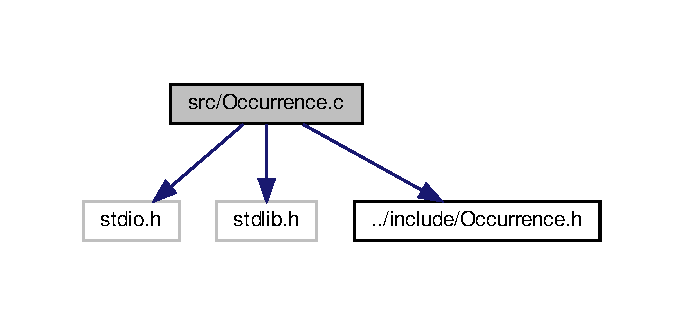
\includegraphics[width=328pt]{_occurrence_8c__incl}
\end{center}
\end{figure}
\subsection*{Functions}
\begin{DoxyCompactItemize}
\item 
\hyperlink{struct_element}{Element} $\ast$ \hyperlink{_occurrence_8c_a7dbd8ad59e7c54573c3cc6554104ec24}{create\+\_\+\+Element} (char letter)
\begin{DoxyCompactList}\small\item\em Create an \hyperlink{struct_element}{Element} object. \end{DoxyCompactList}\item 
void \hyperlink{_occurrence_8c_a7cf8c3bc86fc718bc751012a3ea1bae8}{add\+\_\+occ} (char letter, \hyperlink{struct_element}{Element} $\ast$$\ast$list)
\begin{DoxyCompactList}\small\item\em add one occurrence in the list if the letter exist, else, we create an element at the beginning of the list. \end{DoxyCompactList}\item 
\hyperlink{struct_element}{Element} $\ast$ \hyperlink{_occurrence_8c_a3b8f8fc4b7b66f29fcd36a8e570d65c7}{occurrence} (char $\ast$texte)
\begin{DoxyCompactList}\small\item\em read text file and use add\+\_\+occ to. add letter by letter an occurence to the list of all occurrences. \end{DoxyCompactList}\item 
int \hyperlink{_occurrence_8c_a4a38bc5a9956d58acc78b493668f9e9c}{list\+\_\+size} (\hyperlink{struct_element}{Element} $\ast$l)
\begin{DoxyCompactList}\small\item\em Function who return size of a list. \end{DoxyCompactList}\item 
void \hyperlink{_occurrence_8c_a7bbb9c9a86ff13775d620292f2b29f61}{print\+\_\+list} (\hyperlink{struct_element}{Element} $\ast$list)
\begin{DoxyCompactList}\small\item\em Function to print a list information of a list. \end{DoxyCompactList}\end{DoxyCompactItemize}


\subsection{Function Documentation}
\mbox{\Hypertarget{_occurrence_8c_a7cf8c3bc86fc718bc751012a3ea1bae8}\label{_occurrence_8c_a7cf8c3bc86fc718bc751012a3ea1bae8}} 
\index{Occurrence.\+c@{Occurrence.\+c}!add\+\_\+occ@{add\+\_\+occ}}
\index{add\+\_\+occ@{add\+\_\+occ}!Occurrence.\+c@{Occurrence.\+c}}
\subsubsection{\texorpdfstring{add\+\_\+occ()}{add\_occ()}}
{\footnotesize\ttfamily void add\+\_\+occ (\begin{DoxyParamCaption}\item[{char}]{letter,  }\item[{\hyperlink{struct_element}{Element} $\ast$$\ast$}]{list }\end{DoxyParamCaption})}



add one occurrence in the list if the letter exist, else, we create an element at the beginning of the list. 

\begin{DoxyNote}{Note}
so it modify a list. 
\end{DoxyNote}

\begin{DoxyParams}{Parameters}
{\em letter} & the char to add in the new \hyperlink{struct_element}{Element}. \\
\hline
{\em list} & list we modify,so need double pointer. \\
\hline
\end{DoxyParams}
\mbox{\Hypertarget{_occurrence_8c_a7dbd8ad59e7c54573c3cc6554104ec24}\label{_occurrence_8c_a7dbd8ad59e7c54573c3cc6554104ec24}} 
\index{Occurrence.\+c@{Occurrence.\+c}!create\+\_\+\+Element@{create\+\_\+\+Element}}
\index{create\+\_\+\+Element@{create\+\_\+\+Element}!Occurrence.\+c@{Occurrence.\+c}}
\subsubsection{\texorpdfstring{create\+\_\+\+Element()}{create\_Element()}}
{\footnotesize\ttfamily \hyperlink{struct_element}{Element}$\ast$ create\+\_\+\+Element (\begin{DoxyParamCaption}\item[{char}]{letter }\end{DoxyParamCaption})}



Create an \hyperlink{struct_element}{Element} object. 

\begin{DoxyNote}{Note}
occ initialized at 1. 
\end{DoxyNote}

\begin{DoxyParams}{Parameters}
{\em letter} & the char to add in the new \hyperlink{struct_element}{Element}. \\
\hline
\end{DoxyParams}
\begin{DoxyReturn}{Returns}
Element$\ast$. 
\end{DoxyReturn}
\mbox{\Hypertarget{_occurrence_8c_a4a38bc5a9956d58acc78b493668f9e9c}\label{_occurrence_8c_a4a38bc5a9956d58acc78b493668f9e9c}} 
\index{Occurrence.\+c@{Occurrence.\+c}!list\+\_\+size@{list\+\_\+size}}
\index{list\+\_\+size@{list\+\_\+size}!Occurrence.\+c@{Occurrence.\+c}}
\subsubsection{\texorpdfstring{list\+\_\+size()}{list\_size()}}
{\footnotesize\ttfamily int list\+\_\+size (\begin{DoxyParamCaption}\item[{\hyperlink{struct_element}{Element} $\ast$}]{l }\end{DoxyParamCaption})}



Function who return size of a list. 


\begin{DoxyParams}{Parameters}
{\em l,list} & of \hyperlink{struct_element}{Element}. \\
\hline
\end{DoxyParams}
\begin{DoxyReturn}{Returns}
int, the size of the list. 
\end{DoxyReturn}
\mbox{\Hypertarget{_occurrence_8c_a3b8f8fc4b7b66f29fcd36a8e570d65c7}\label{_occurrence_8c_a3b8f8fc4b7b66f29fcd36a8e570d65c7}} 
\index{Occurrence.\+c@{Occurrence.\+c}!occurrence@{occurrence}}
\index{occurrence@{occurrence}!Occurrence.\+c@{Occurrence.\+c}}
\subsubsection{\texorpdfstring{occurrence()}{occurrence()}}
{\footnotesize\ttfamily \hyperlink{struct_element}{Element}$\ast$ occurrence (\begin{DoxyParamCaption}\item[{char $\ast$}]{texte }\end{DoxyParamCaption})}



read text file and use add\+\_\+occ to. add letter by letter an occurence to the list of all occurrences. 


\begin{DoxyParams}{Parameters}
{\em texte} & file in wich we read char by char. \\
\hline
\end{DoxyParams}
\begin{DoxyReturn}{Returns}
Element$\ast$, the list of all occurrences. 
\end{DoxyReturn}
\mbox{\Hypertarget{_occurrence_8c_a7bbb9c9a86ff13775d620292f2b29f61}\label{_occurrence_8c_a7bbb9c9a86ff13775d620292f2b29f61}} 
\index{Occurrence.\+c@{Occurrence.\+c}!print\+\_\+list@{print\+\_\+list}}
\index{print\+\_\+list@{print\+\_\+list}!Occurrence.\+c@{Occurrence.\+c}}
\subsubsection{\texorpdfstring{print\+\_\+list()}{print\_list()}}
{\footnotesize\ttfamily void print\+\_\+list (\begin{DoxyParamCaption}\item[{\hyperlink{struct_element}{Element} $\ast$}]{list }\end{DoxyParamCaption})}



Function to print a list information of a list. 

\begin{DoxyNote}{Note}
Print letter and number of occurrence. 
\end{DoxyNote}

\begin{DoxyParams}{Parameters}
{\em list,list} & of \hyperlink{struct_element}{Element}. \\
\hline
\end{DoxyParams}

%--- End generated contents ---

% Index
\backmatter
\newpage
\phantomsection
\clearemptydoublepage
\addcontentsline{toc}{chapter}{Index}
\printindex

\end{document}
